\documentclass[12pt,a4paper]{article}

\usepackage[margin=1in]{geometry}
\usepackage{amsmath,amssymb,amsthm}
\usepackage{booktabs}
\usepackage{graphicx}
\usepackage{hyperref}
\usepackage{microtype}
\usepackage{parskip}
\usepackage{enumitem}
\usepackage{float}
\usepackage{caption}
\usepackage{subcaption}
\usepackage{xcolor}
\usepackage{array}
\usepackage[numbers,sort&compress]{natbib}

\graphicspath{{./report_figures/}}

\hypersetup{
  colorlinks=true,
  linkcolor=blue!60!black,
  citecolor=blue!60!black,
  urlcolor=blue!60!black,
}

\title{%
  \Large\textbf{Stochastic Calculus and Its Applications in Finance}\\[0.5em]
  \large Course Project Report
}
\author{Aditya Nagarsekar}
\date{}

\begin{document}
\maketitle
\thispagestyle{empty}
\newpage
\tableofcontents
\newpage

% ═════════════════════════════════════════════════════════════════════════════
\section*{Abstract}
\addcontentsline{toc}{section}{Abstract}
% ═════════════════════════════════════════════════════════════════════════════

Options are contracts whose value depends on the random future path of an
underlying asset.  Pricing and hedging them requires a model for that path,
mathematical tools to extract prices and sensitivities, and in practice an
estimate of the model's key parameter, volatility.  This project addresses all
three layers simultaneously.

\textbf{Component~1} trains a reinforcement learning (RL) agent via Proximal
Policy Optimization (PPO) to hedge a European call option under geometric
Brownian motion (GBM).  Black-Scholes-Merton (BSM) delta is provably optimal
under GBM.  The agent, never shown the BSM formula, independently recovers it
with a state-aligned hedge-ratio correlation of \textbf{0.960}.  Three
theory-motivated extensions are then developed: a Heston stochastic-volatility
environment (RL diverges from BSM delta as theory predicts, corr drops to
0.840), an It\^{o}-decomposed reward that removes the irreducible gamma term
from the training signal ($-2.6\%$ MAE, $-13\%$ TC), and a gamma-aware
observation ($-31\%$ TC vs.\ baseline).

\textbf{Component~2} forecasts one-step-ahead realised volatility using a
two-layer stacked LSTM, beating a rolling GARCH(1,1) benchmark by \textbf{27\%
on RMSE} and \textbf{47\% on MAE} out-of-sample.  Forecasts feed a BSM
pricing pipeline; Vega sensitivity analysis quantifies how vol errors propagate
to pricing errors.

\textbf{Integration} feeds the LSTM vol schedule into the hedging environment,
connecting both components end-to-end.  The LSTM-guided agent achieves the
lowest transaction cost of all RL variants (0.102) at a modest MAE cost.

All three components share the same mathematical spine: It\^{o}'s lemma, the
BSM Greeks ($\Delta$, $\Gamma$, Vega), and the GBM/Heston stochastic
differential equations.

% ═════════════════════════════════════════════════════════════════════════════
\section{Introduction}
\label{sec:intro}
% ═════════════════════════════════════════════════════════════════════════════

\subsection{Motivation}

The Black-Scholes-Merton formula \citep{Black1973} gives a closed-form price
for European options and the exact hedge ratio under idealised assumptions:
continuous trading, constant volatility, no transaction costs.  Three of those
assumptions fail in practice:

\begin{enumerate}
  \item \textbf{Discrete rebalancing with transaction costs.}  Continuous
        hedging is theoretically costless; daily or weekly hedging incurs
        proportional costs that must be balanced against hedging accuracy.  The
        optimal discrete policy is not BSM delta and has no known closed form.

  \item \textbf{Stochastic volatility.}  Equity index vol is random and
        mean-reverting.  BSM delta computed at a constant $\sigma$ is no longer
        optimal when $\sigma$ itself is a stochastic process.

  \item \textbf{Unknown volatility.}  Even if BSM were the right model, $\sigma$
        is unobservable and must be estimated.  Forecast accuracy translates
        directly into pricing accuracy via the Vega Greek.
\end{enumerate}

This project addresses all three within a unified framework.

\subsection{Project Structure and Mathematical Thread}

\begin{description}[leftmargin=2cm]
  \item[Component~1] RL agent learns optimal discrete-time hedge; tested under
        GBM and Heston stochastic vol.  Novel reward and observation design
        motivated by It\^{o}'s lemma.
  \item[Component~2] LSTM forecasts NIFTY~50 volatility, outperforms GARCH(1,1).
        Forecasts drive a BSM pricing horse-race; Vega links forecast error to
        pricing error.
  \item[Integration] LSTM vol schedule replaces fixed $\sigma$ in the hedging
        environment; end-to-end test of the pipeline.
\end{description}

Three quantities from It\^{o}'s lemma appear throughout:
$\Delta = \partial V/\partial S$ (hedging target for Component~1),
$\Gamma = \partial^2 V/\partial S^2$ (novel reward and observation design), and
$\mathcal{V} = \partial V/\partial\sigma$ --- Vega (propagates LSTM forecast
errors into pricing errors in Component~2).

\subsection{Baselines}
\label{sec:baselines}

Every experiment is compared against well-defined baselines.  These are
summarised here for clarity; each is described in full detail in the relevant
section.

\begin{table}[H]
  \centering
  \caption{All baselines used in the project.}
  \label{tab:baselines}
  \begin{tabular}{lp{7.5cm}l}
    \toprule
    Baseline & Description & Used in \\
    \midrule
    \textbf{BSM delta (daily)} &
      At every step, set $\delta_t = \Delta^* = \Phi(d_1)$ evaluated at the
      current $(S_t, \tau_t, \sigma)$.  No learning; rebalances 21 times per
      episode.  Theoretically optimal under GBM with no TC. &
      \S\ref{sec:p1}, \S\ref{sec:integration} \\[6pt]

    \textbf{BSM delta (weekly)} &
      Same formula, but rebalances every 5 steps (4 trades per episode).
      Reduces TC at the cost of hedging accuracy. &
      \S\ref{sec:p1} \\[6pt]

    \textbf{RL, constant $\sigma$} &
      PPO agent trained with a fixed $\sigma=0.20$ in the environment.
      Primary RL baseline against which novel extensions are compared. &
      \S\ref{sec:p1}, \S\ref{sec:integration} \\[6pt]

    \textbf{Exp A: GBM + MSE reward} &
      Same as ``RL constant $\sigma$'' but re-run inside the novel experiment
      framework (300k steps, 1000 eval episodes) to give a consistent
      comparison baseline for experiments B--E. &
      \S\ref{sec:novel} \\[6pt]

    \textbf{GARCH(1,1)} &
      Rolling expanding-window GARCH fitted at every test step with no
      look-ahead.  Industry-standard conditional vol model; 40-year benchmark. &
      \S\ref{sec:p3} \\[6pt]

    \textbf{Historical rolling vol} &
      21-day rolling standard deviation of log-returns, annualised.
      Simplest possible vol estimate; requires no model fitting. &
      \S\ref{sec:p3} \\[6pt]

    \textbf{Implied vol} &
      Vol recovered from proxy market prices via BSM inversion
      (Brent's method).  Represents the ``market's'' estimate and trivially
      achieves zero pricing error against its own proxy prices. &
      \S\ref{sec:p3} \\
    \bottomrule
  \end{tabular}
\end{table}

The hierarchy of baselines in Component~1 is:
BSM~daily $>$ BSM~weekly $>$ RL~constant~$\sigma$, where ``$>$'' means
lower hedging MAE but typically higher TC.
The RL agent's goal is to identify the best point on this MAE-vs-TC
Pareto frontier; the novel experiments explore whether improved reward
signals or richer observations shift that frontier favourably.

% ═════════════════════════════════════════════════════════════════════════════
\section{Component 1: Reinforcement Learning Delta Hedging}
\label{sec:p1}
% ═════════════════════════════════════════════════════════════════════════════

\subsection{Theoretical Background}
\label{sec:p1_theory}

\subsubsection{Geometric Brownian Motion}

Under the risk-neutral measure $\mathbb{Q}$, the stock price $S_t$ satisfies
\begin{equation}
  dS_t = r\,S_t\,dt + \sigma\,S_t\,dW_t,
  \label{eq:gbm}
\end{equation}
where $r$ is the risk-free rate, $\sigma > 0$ constant volatility, and $W_t$
a standard Brownian motion.
Applying It\^{o}'s formula to $f(S) = \ln S$ gives
\begin{equation}
  d\ln S_t = \bigl(r - \tfrac{1}{2}\sigma^2\bigr)dt + \sigma\,dW_t,
  \label{eq:log_gbm}
\end{equation}
so $\ln(S_t/S_0) \sim \mathcal{N}((r-\tfrac12\sigma^2)t,\;\sigma^2 t)$.
The exact solution over one discrete step $\Delta t$ is therefore:
\begin{equation}
  S_{t+\Delta t} = S_t\exp\!\bigl((r-\tfrac12\sigma^2)\Delta t
                   + \sigma\sqrt{\Delta t}\,Z\bigr),
  \quad Z\sim\mathcal{N}(0,1).
  \label{eq:log_euler}
\end{equation}
This is the log-Euler step used in the environment --- exact for GBM, not an
approximation.

\subsubsection{Black-Scholes-Merton Price and Greeks}

For a European call with strike $K$ and maturity $T$:
\begin{equation}
  V(S,\tau) = S\,\Phi(d_1) - Ke^{-r\tau}\Phi(d_2), \quad
  d_{1,2} = \frac{\ln(S/K)+(r\pm\tfrac12\sigma^2)\tau}{\sigma\sqrt{\tau}},
  \label{eq:bsm}
\end{equation}
with $\tau = T-t$.  The Greeks are:
\begin{align}
  \Delta^* &= \frac{\partial V}{\partial S} = \Phi(d_1), \label{eq:delta}\\
  \Gamma   &= \frac{\partial^2 V}{\partial S^2}
             = \frac{\phi(d_1)}{S\sigma\sqrt{\tau}}, \label{eq:gamma}\\
  \mathcal{V} &= \frac{\partial V}{\partial\sigma}
               = S\,\phi(d_1)\sqrt{\tau}. \label{eq:vega}
\end{align}
Figure~\ref{fig:delta_surface} shows how $\Delta^*$ varies across moneyness
and time-to-expiry.  The RL agent must learn this surface from reward alone.

\begin{figure}[H]
  \centering
  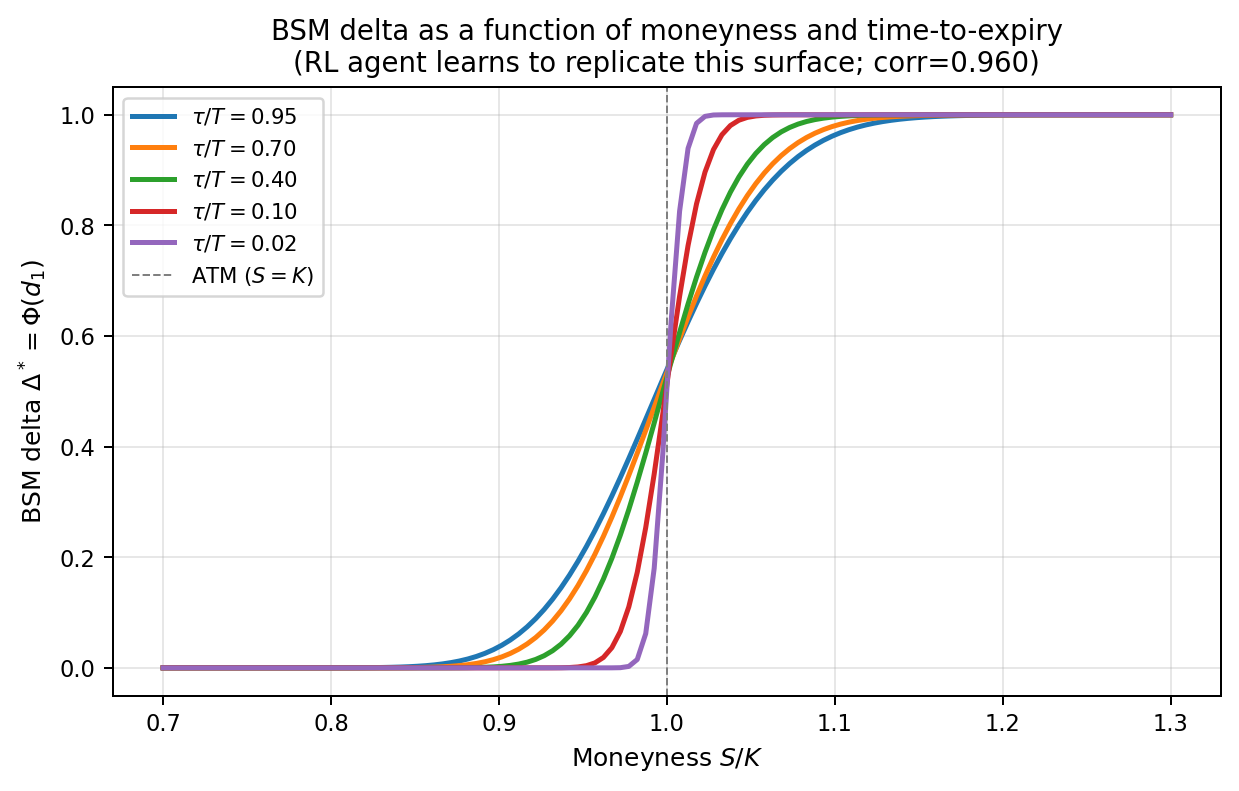
\includegraphics[width=0.72\textwidth]{fig_bsm_delta_surface.png}
  \caption{BSM delta $\Delta^* = \Phi(d_1)$ as a function of moneyness $S/K$
           and normalised time-to-expiry $\tau/T$ ($\sigma=0.20$).
           The agent's observation space is spanned by these variables;
           the surface represents the theoretically optimal action at each
           state.}
  \label{fig:delta_surface}
\end{figure}

\subsubsection{It\^{o}'s Lemma and the Hedging Error Decomposition}

Applying It\^{o}'s lemma to $V(S_t, t)$:
\begin{equation}
  dV = \frac{\partial V}{\partial t}dt
     + \underbrace{\frac{\partial V}{\partial S}}_{\Delta^*}dS
     + \frac{1}{2}\underbrace{\frac{\partial^2 V}{\partial S^2}}_{\Gamma}(dS)^2.
\end{equation}
A hedge holds $\delta$ shares.  The one-step P\&L of the hedged position is:
\begin{equation}
  \varepsilon_t = \delta\,\Delta S - \Delta V
  = \underbrace{(\delta - \Delta^*)\Delta S}_{\text{controllable}}
  \;-\;\underbrace{\tfrac{1}{2}\Gamma\bigl[(\Delta S)^2 - \sigma^2 S^2\Delta t\bigr]}_{\text{irreducible gamma noise}}.
  \label{eq:hedge_error}
\end{equation}
The gamma term is zero in expectation (since $\mathbb{E}[(\Delta S)^2]
= \sigma^2 S^2\Delta t$ under GBM) but non-zero in any realisation.
\emph{No choice of $\delta$ eliminates it.}
This decomposition motivates the It\^{o} reward (Section~\ref{sec:ito_reward})
and the gamma observation (Section~\ref{sec:gamma_obs}).
Figure~\ref{fig:ito_decomp} shows the empirical distributions of all three
terms over 500 simulated episodes.

\begin{figure}[H]
  \centering
  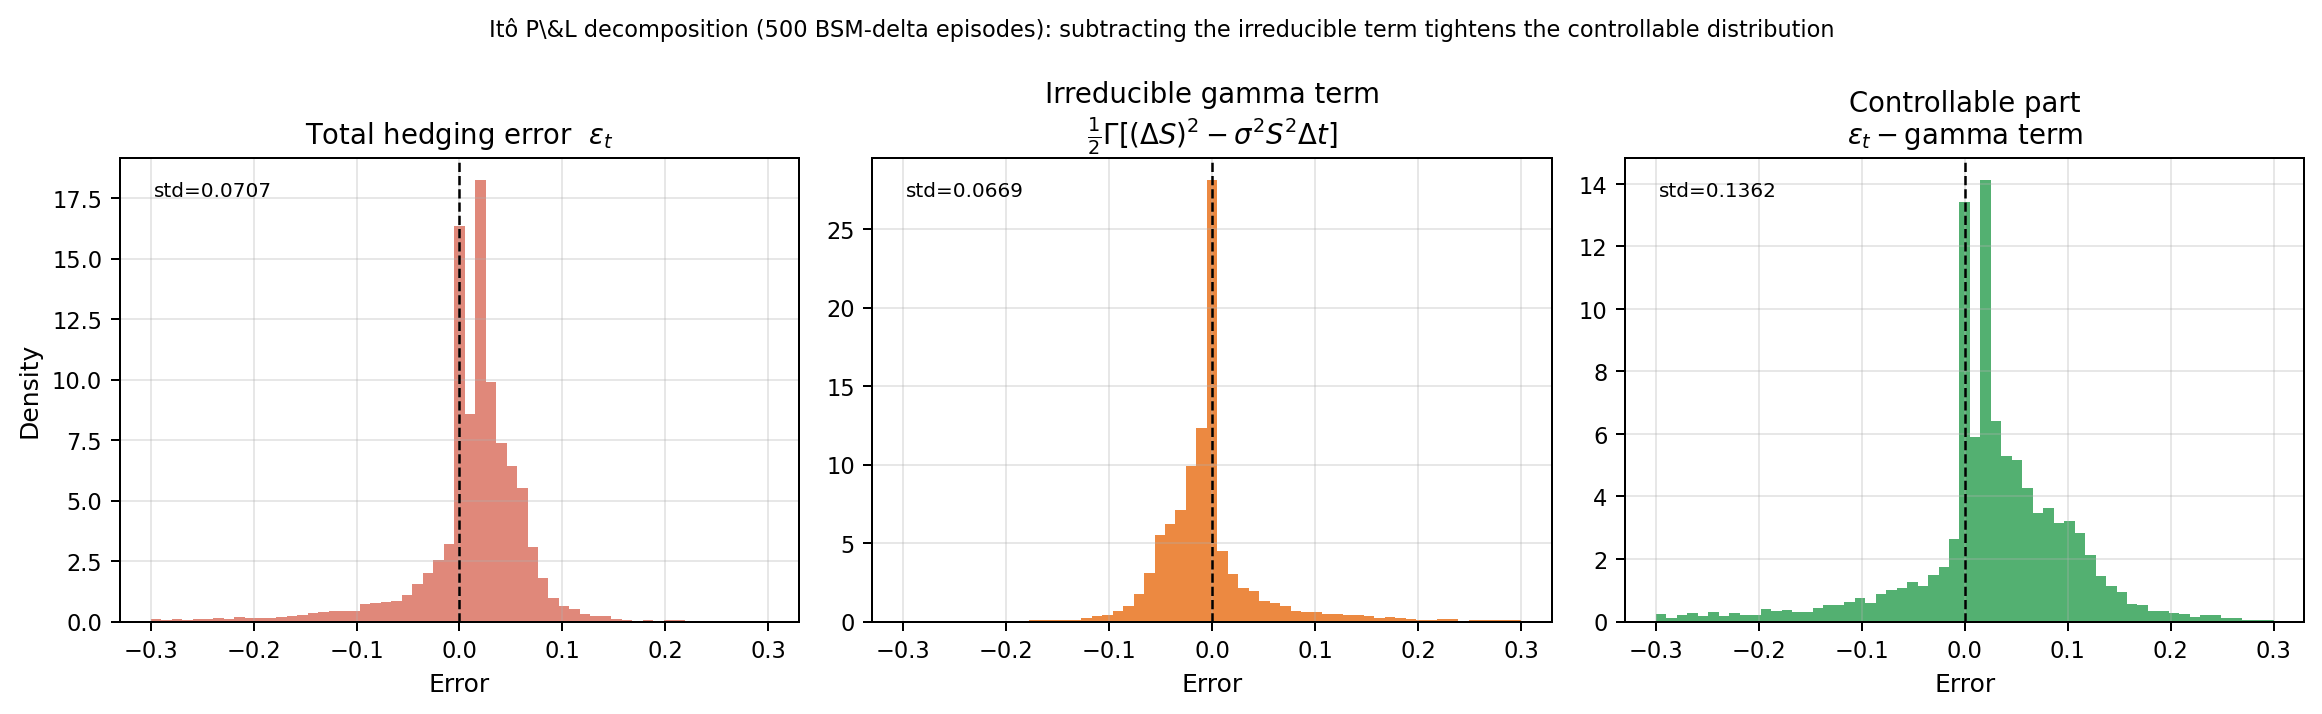
\includegraphics[width=\textwidth]{fig_ito_decomp.png}
  \caption{Itô P\&L decomposition over 500 simulated BSM-delta episodes.
           \emph{Left:} total hedging error $\varepsilon_t$.
           \emph{Centre:} irreducible gamma term (same variance as total).
           \emph{Right:} controllable part after subtracting the gamma term.
           Note the tighter distribution on the right --- when the gamma noise
           is removed, the residual is the signal the RL agent can actually
           act on.}
  \label{fig:ito_decomp}
\end{figure}

\subsubsection{Why BSM Delta is Optimal Under GBM}

Under GBM with no transaction costs, $\Delta^* = \Phi(d_1)$ minimises
$\mathbb{E}[\varepsilon_t^2]$ at each step by setting the controllable term in
\eqref{eq:hedge_error} to zero in expectation.
With transaction costs, the optimal policy is more conservative and has no
closed form.  This is precisely the problem the RL agent solves.

\subsection{Environment Design}

The \texttt{HedgingEnv} gymnasium environment simulates hedging a European call
over $n=21$ discrete steps ($T=21/252$ years, one trading month).

\begin{itemize}
  \item \textbf{Observation:} $\mathbf{o}_t = [S_t/K,\;\tau_t/T,\;\delta_{t-1}]$
        --- three numbers sufficient in principle to compute BSM delta.
  \item \textbf{Action:} $\delta_t \in [0,1]$, the hedge ratio.
  \item \textbf{Dynamics:} Exact log-Euler GBM step \eqref{eq:log_euler}.
  \item \textbf{Reward:} $r_t = -\varepsilon_t^2 - \kappa|\delta_t-\delta_{t-1}|S_t$,
        where $\kappa=0.001$ is the proportional transaction-cost rate.
  \item \textbf{Episode start:} $S_0 \sim \text{Uniform}(0.9K,\;1.1K)$ to
        expose the agent to a range of moneyness values.
\end{itemize}

\subsection{PPO Agent and Training}

Proximal Policy Optimization \citep{Schulman2017} uses a two-hidden-layer MLP
policy (128--64 units, Tanh), learning rate $10^{-4}$, rollout $n=512$, batch
size 128, 10 epochs per update, $\gamma=0.99$, trained for 300\,000 steps
across 4 parallel environments.

\subsection{Results}
\label{sec:p1_results}

\begin{table}[H]
  \centering
  \caption{Simulated-environment hedging results (1\,000 episodes, $\sigma=0.20$,
           $\kappa=0.001$).}
  \label{tab:p1_main}
  \begin{tabular}{lccc}
    \toprule
    Strategy & MAE & Mean TC & RL--BSM $\delta$ corr \\
    \midrule
    BSM delta (daily)  & \textbf{0.284} & 0.146 & --- \\
    BSM delta (weekly) & 0.499 & 0.098 & --- \\
    RL (PPO)           & 0.748 & 0.127 & \textbf{0.960} \\
    \bottomrule
  \end{tabular}
\end{table}

\begin{figure}[H]
  \centering
  \begin{subfigure}[t]{0.52\textwidth}
    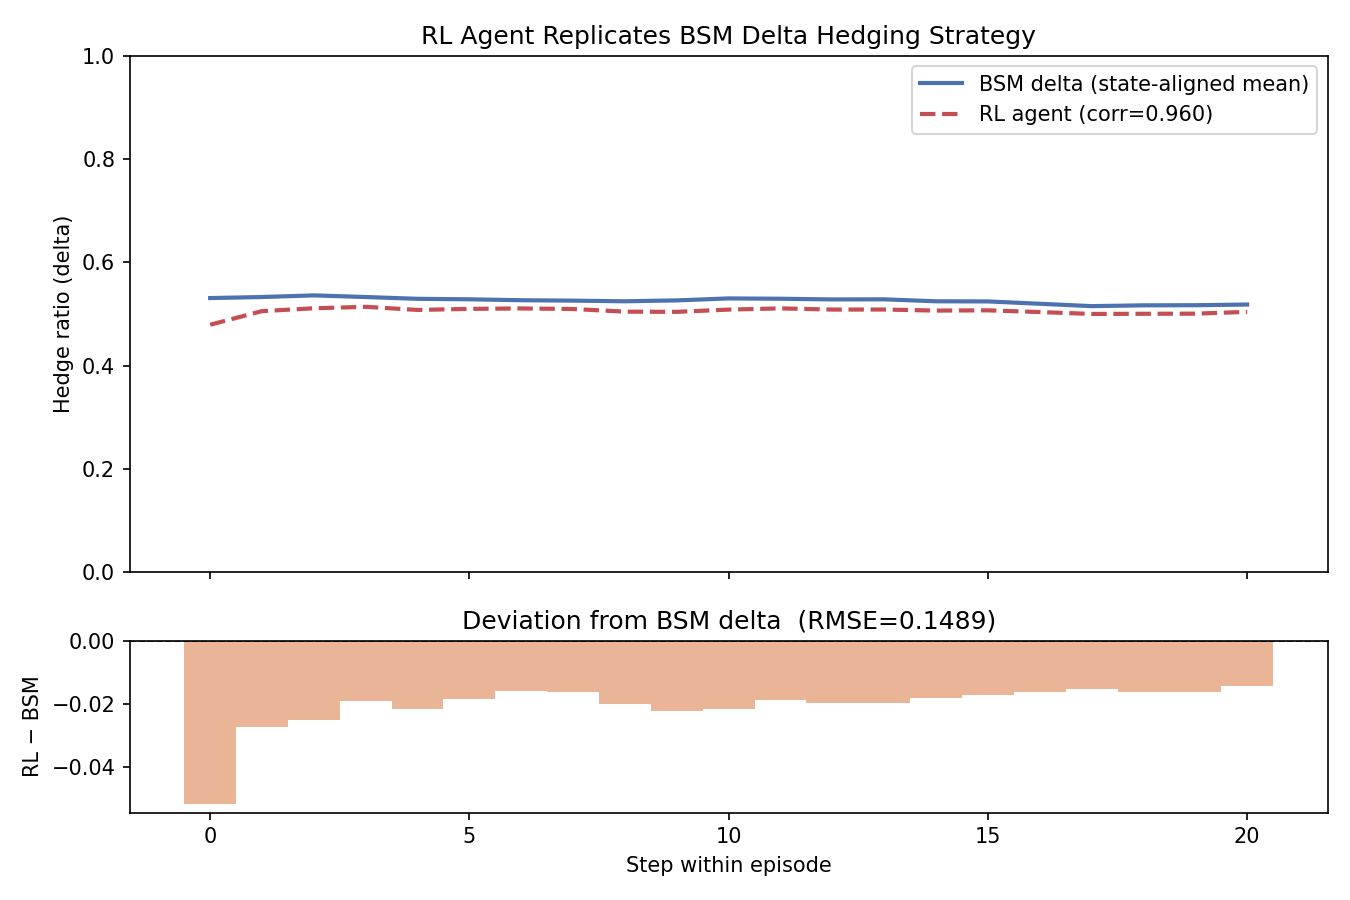
\includegraphics[width=\textwidth]{fig_p1_hedge_ratios.png}
    \caption{Mean hedge ratio over an episode.  RL closely tracks BSM daily;
             the small systematic gap reflects TC-induced under-rebalancing.}
    \label{fig:hedge_ratios}
  \end{subfigure}
  \hfill
  \begin{subfigure}[t]{0.46\textwidth}
    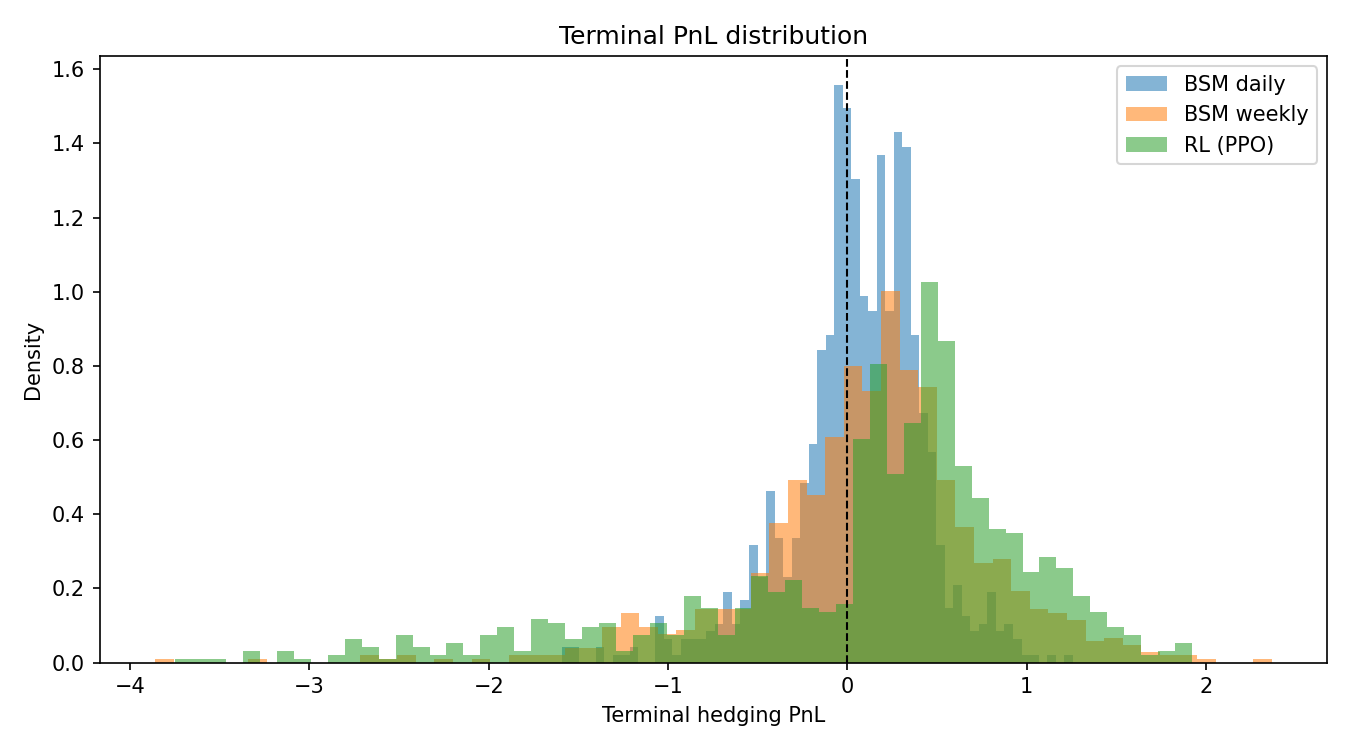
\includegraphics[width=\textwidth]{fig_p1_pnl_dist.png}
    \caption{Terminal P\&L distributions.  BSM daily is tightest (lowest
             variance); RL is wider but centred closer to zero than BSM weekly.}
    \label{fig:pnl_dist}
  \end{subfigure}
  \caption{Component~1 main results.}
\end{figure}

\paragraph{RL replicates BSM delta (corr = 0.960).}
The state-aligned correlation is the key result.  At each step of each
evaluation episode, BSM delta is recomputed at the actual $(S_t,\tau_t)$
decoded from the observation ($S_t = o_t[0]\cdot K$, $\tau_t = o_t[1]\cdot T$)
and correlated with the RL action.  A correlation of 0.960 confirms the agent
learned the $\Phi(d_1)$ surface (Figure~\ref{fig:delta_surface}) purely from
the reward signal.

\paragraph{Why RL MAE exceeds BSM daily.}
The agent is penalised for transaction costs and learns to rebalance less
frequently.  BSM daily achieves MAE 0.284 at cost 0.146; the RL agent achieves
MAE 0.748 at cost 0.127.  The MAE gap reflects the cost-accuracy trade-off,
not suboptimality.  Figure~\ref{fig:hedging_error_box} shows the error
distribution by strategy.

\begin{figure}[H]
  \centering
  \begin{subfigure}[t]{0.52\textwidth}
    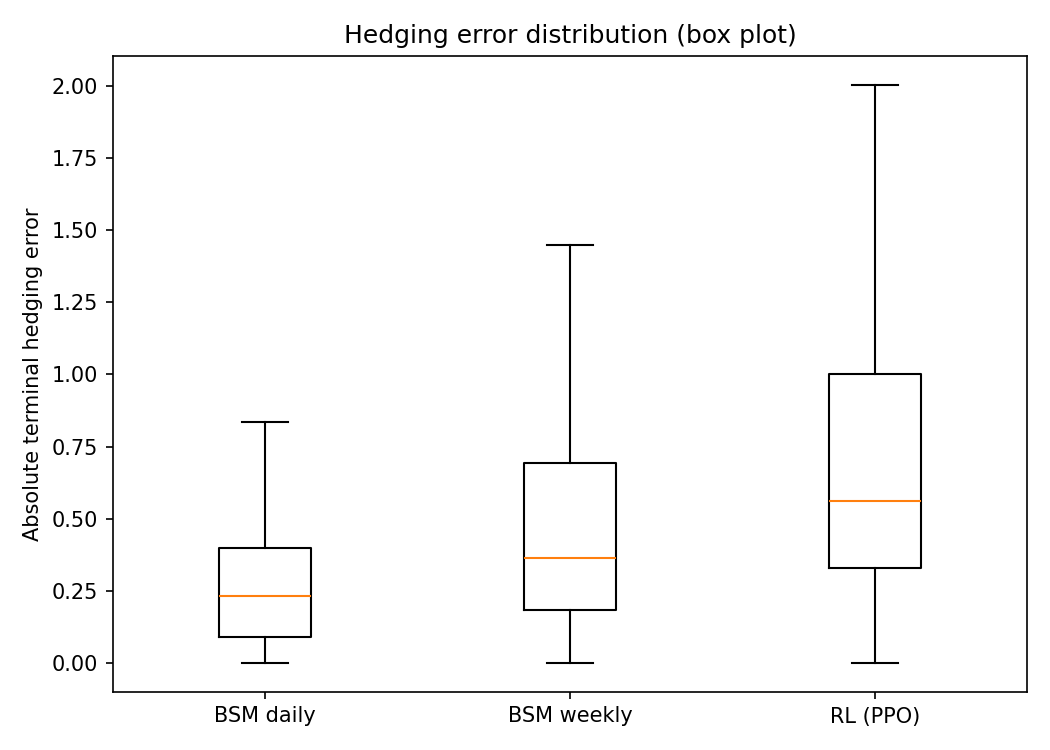
\includegraphics[width=\textwidth]{fig_p1_error_boxplot.png}
    \caption{Hedging error distributions by strategy.  BSM daily has the
             tightest interquartile range; RL has heavier tails reflecting
             infrequent rebalancing.}
    \label{fig:hedging_error_box}
  \end{subfigure}
  \hfill
  \begin{subfigure}[t]{0.46\textwidth}
    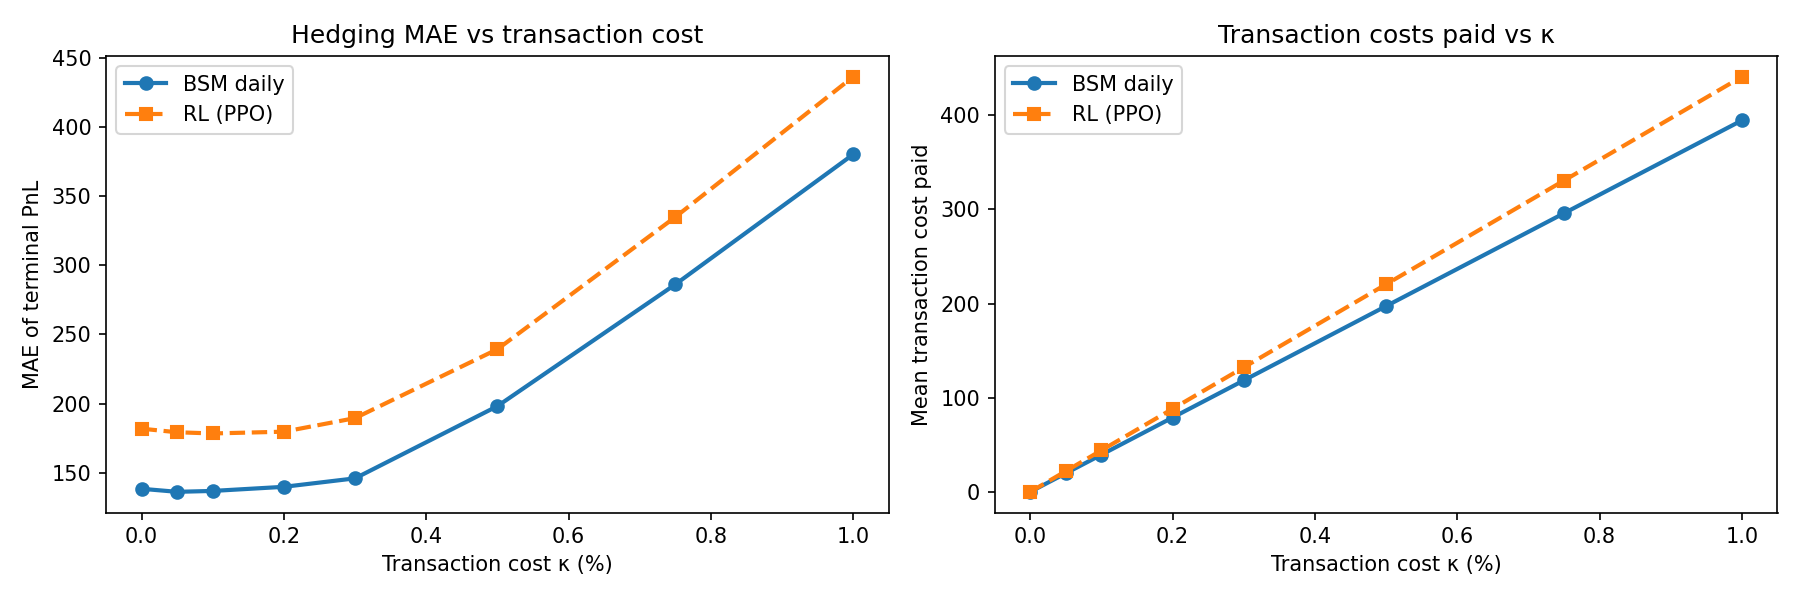
\includegraphics[width=\textwidth]{fig_tc_sensitivity.png}
    \caption{MAE vs.\ transaction-cost rate $\kappa$.  Both strategies degrade
             proportionally; RL maintains a roughly constant relative gap.}
    \label{fig:tc_sensitivity}
  \end{subfigure}
  \caption{Hedging error structure and cost sensitivity.}
\end{figure}

\paragraph{Real-path evaluation.}
When strategies are evaluated on historical NIFTY~50 price paths, absolute P\&L
scales are much larger (genuine vol spikes):

\begin{table}[H]
  \centering
  \caption{Real-path evaluation on NIFTY 50 historical data.}
  \label{tab:p1_real}
  \begin{tabular}{lcccc}
    \toprule
    Strategy & Mean PnL & Std PnL & MAE & Mean TC \\
    \midrule
    BSM daily & $-14.81$ & 226.85 & 136.90 & 39.46 \\
    RL (PPO)  & $\mathbf{-0.38}$ & 293.68 & 178.42 & 44.10 \\
    \bottomrule
  \end{tabular}
\end{table}

\begin{figure}[H]
  \centering
  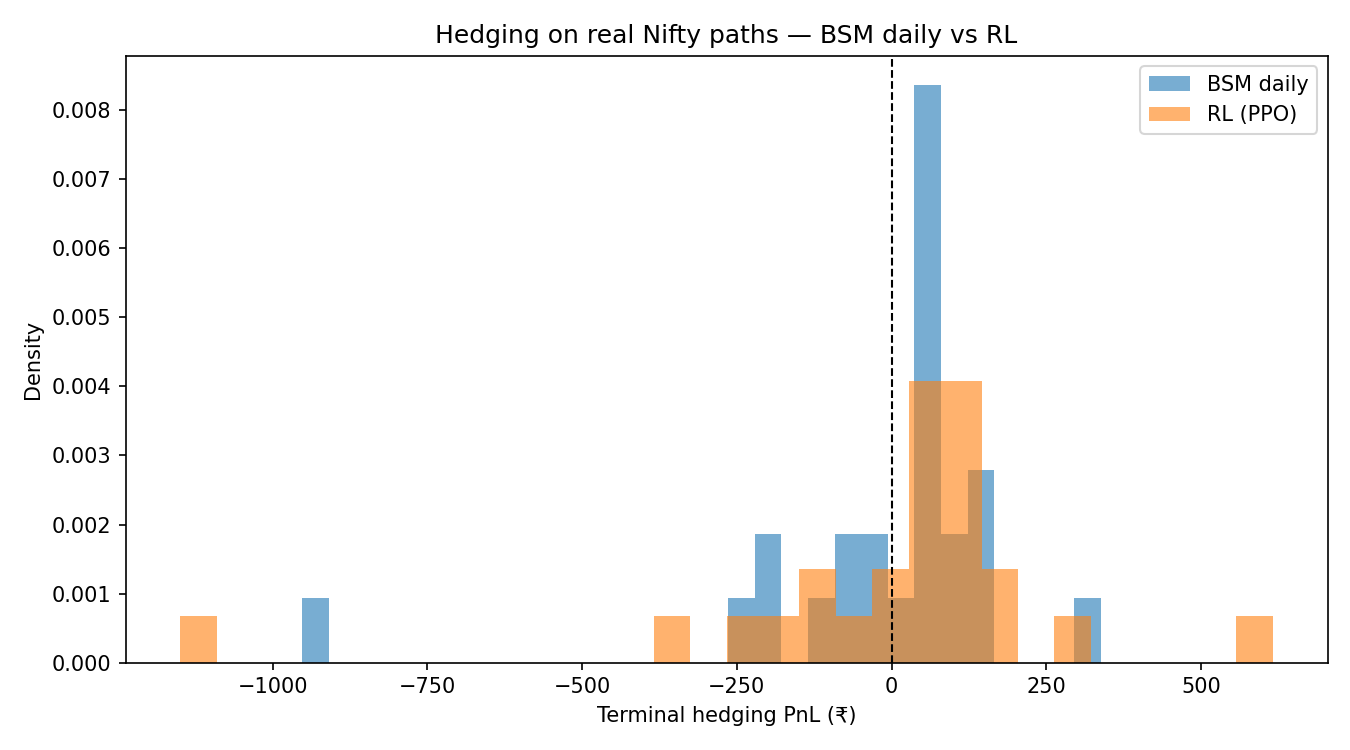
\includegraphics[width=0.72\textwidth]{fig_real_paths_pnl.png}
  \caption{Terminal P\&L distribution on real NIFTY~50 paths.
           RL achieves a near-zero mean P\&L ($-0.38$) vs.\ BSM daily
           ($-14.81$), suggesting it avoids the systematic overhedging that
           BSM exhibits during real vol spikes.  The RL distribution is
           wider because the policy was trained under GBM, not real fat tails.}
  \label{fig:real_paths}
\end{figure}

\subsection{Novel Extensions}
\label{sec:novel}

\subsubsection{Extension 1: Heston Stochastic Volatility}
\label{sec:heston}

\paragraph{Motivation.}
Under GBM, $\sigma$ is constant and BSM delta is optimal.  Under the Heston
model \citep{Heston1993}, the variance $V_t$ itself is stochastic:
\begin{align}
  dS_t &= r\,S_t\,dt + \sqrt{V_t}\,S_t\,dW_1, \label{eq:heston_S}\\
  dV_t &= \kappa(\theta-V_t)\,dt + \xi\sqrt{V_t}\,dW_2, \label{eq:heston_V}\\
  \langle dW_1, dW_2\rangle &= \rho\,dt. \label{eq:heston_rho}
\end{align}
Parameters: $\kappa=2.0$ (mean-reversion), $\theta=0.04$ ($\approx 20\%$ ann.\
vol), $\xi=0.30$ (vol-of-vol), $\rho=-0.70$ (equity leverage effect).
Figure~\ref{fig:heston_paths} shows simulated paths.

\begin{figure}[H]
  \centering
  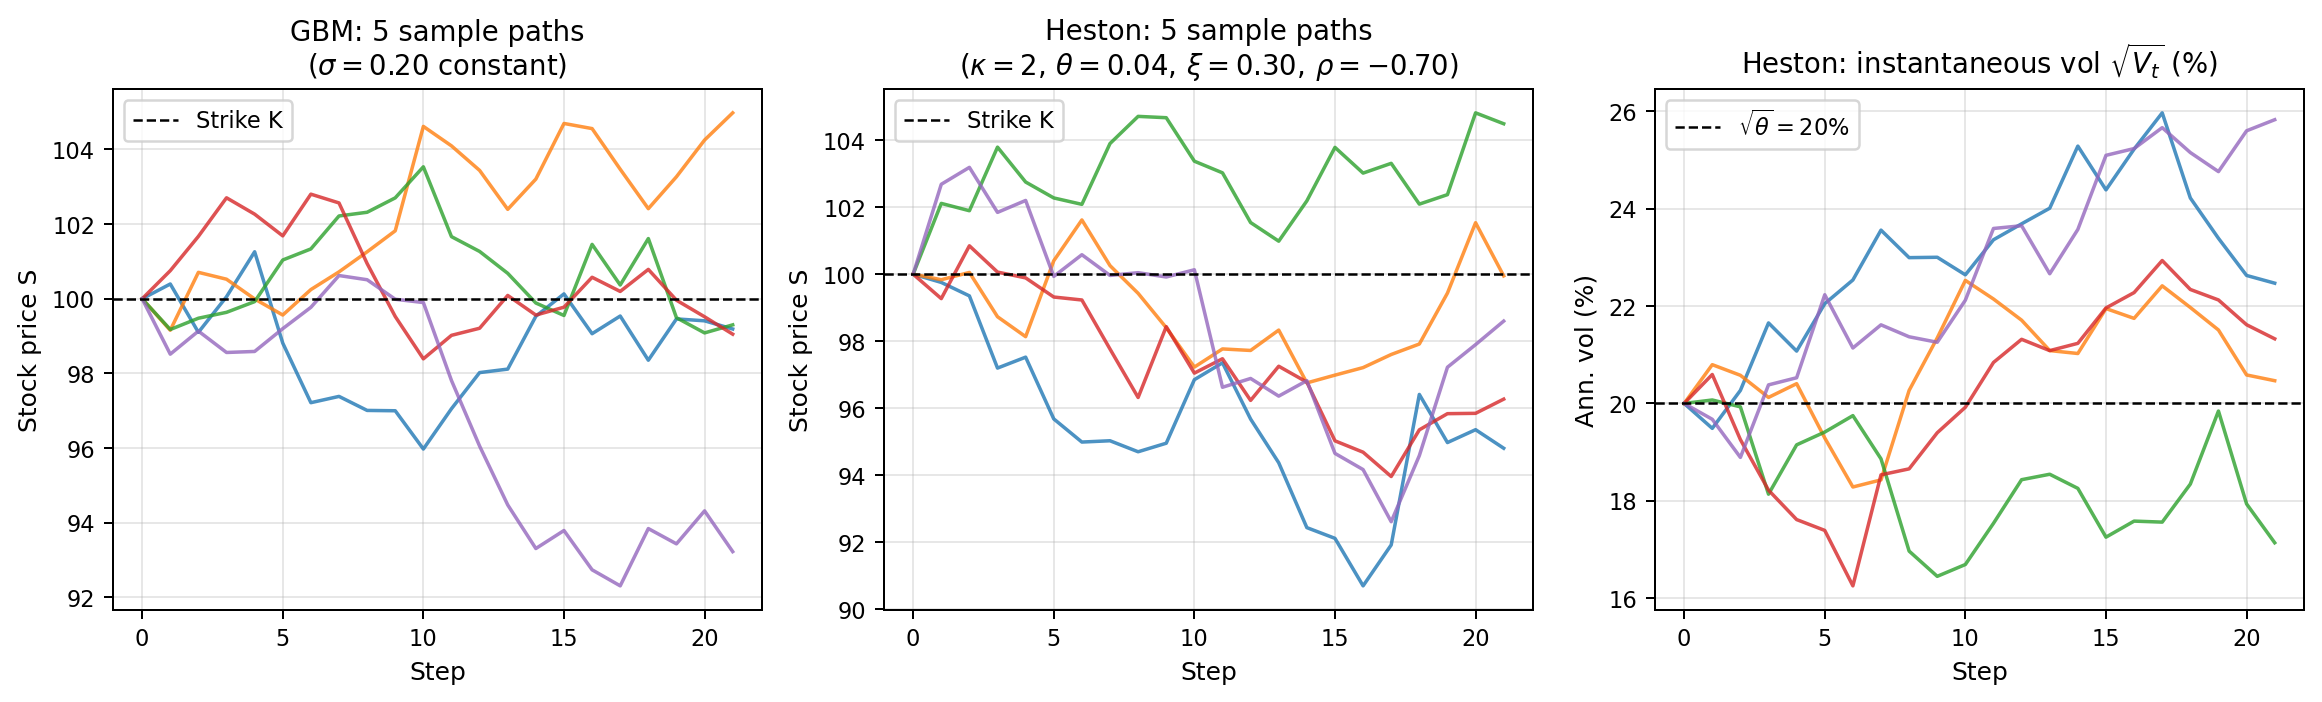
\includegraphics[width=\textwidth]{fig_heston_paths.png}
  \caption{GBM paths (left) vs.\ Heston paths (centre) and the corresponding
           instantaneous vol process $\sqrt{V_t}$ (right).  Under Heston, vol
           clusters and mean-reverts, producing regimes that BSM delta at a
           fixed $\sigma$ cannot adapt to.}
  \label{fig:heston_paths}
\end{figure}

\paragraph{Implementation.}
Variance is discretised with full-truncation Euler--Maruyama:
\begin{equation}
  V_{t+\Delta t} = \max\!\Bigl(
    V_t + \kappa(\theta-V_t)\Delta t
        + \xi\sqrt{V_t}\sqrt{\Delta t}\,Z_2,\;\;10^{-6}
  \Bigr),
\end{equation}
with correlated shocks $W_1=Z_1$, $W_2=\rho Z_1+\sqrt{1-\rho^2}\tilde{Z}$.
The observation is extended to
$\mathbf{o}_t = [S/K,\;\tau/T,\;\delta_{\text{prev}},\;\sqrt{V_t}/\sqrt{\theta}]$,
giving the agent access to the current vol regime.

\subsubsection{Extension 2: It\^{o}-Decomposed Reward}
\label{sec:ito_reward}

\paragraph{Motivation.}
The standard reward penalises $\varepsilon_t^2$, which from
\eqref{eq:hedge_error} mixes the controllable and irreducible parts.
When the gamma term dominates (near-ATM, near-expiry), training noise prevents
the agent from identifying the correct delta.
The It\^{o} reward removes the irreducible part before squaring:
\begin{align}
  \text{gamma P\&L}_t &= \tfrac{1}{2}\Gamma_t
    \bigl[(\Delta S)^2 - \sigma^2 S_t^2\Delta t\bigr], \label{eq:gamma_pnl}\\
  r_t^{\text{It\^{o}}} &= -(\varepsilon_t - \text{gamma P\&L}_t)^2 - \text{tc}_t.
  \label{eq:ito_reward}
\end{align}
The effect is shown in Figure~\ref{fig:ito_decomp}: the controllable
distribution (right panel) has substantially lower variance than the total
error (left panel), providing a cleaner training signal.

\subsubsection{Extension 3: Gamma-Aware Observation}
\label{sec:gamma_obs}

\paragraph{Motivation.}
Dollar-gamma $\Gamma_t S_t$ quantifies the irreducible gamma P\&L's
sensitivity at the current state (see Figure~\ref{fig:gamma_surface}).
It is large near-ATM near-expiry (where hedging errors are amplified) and
nearly zero deep ITM/OTM (where a small delta error costs almost nothing).
BSM delta does not use this information; an RL agent that observes $\Gamma S$
can learn to rebalance only when it matters.

\begin{figure}[H]
  \centering
  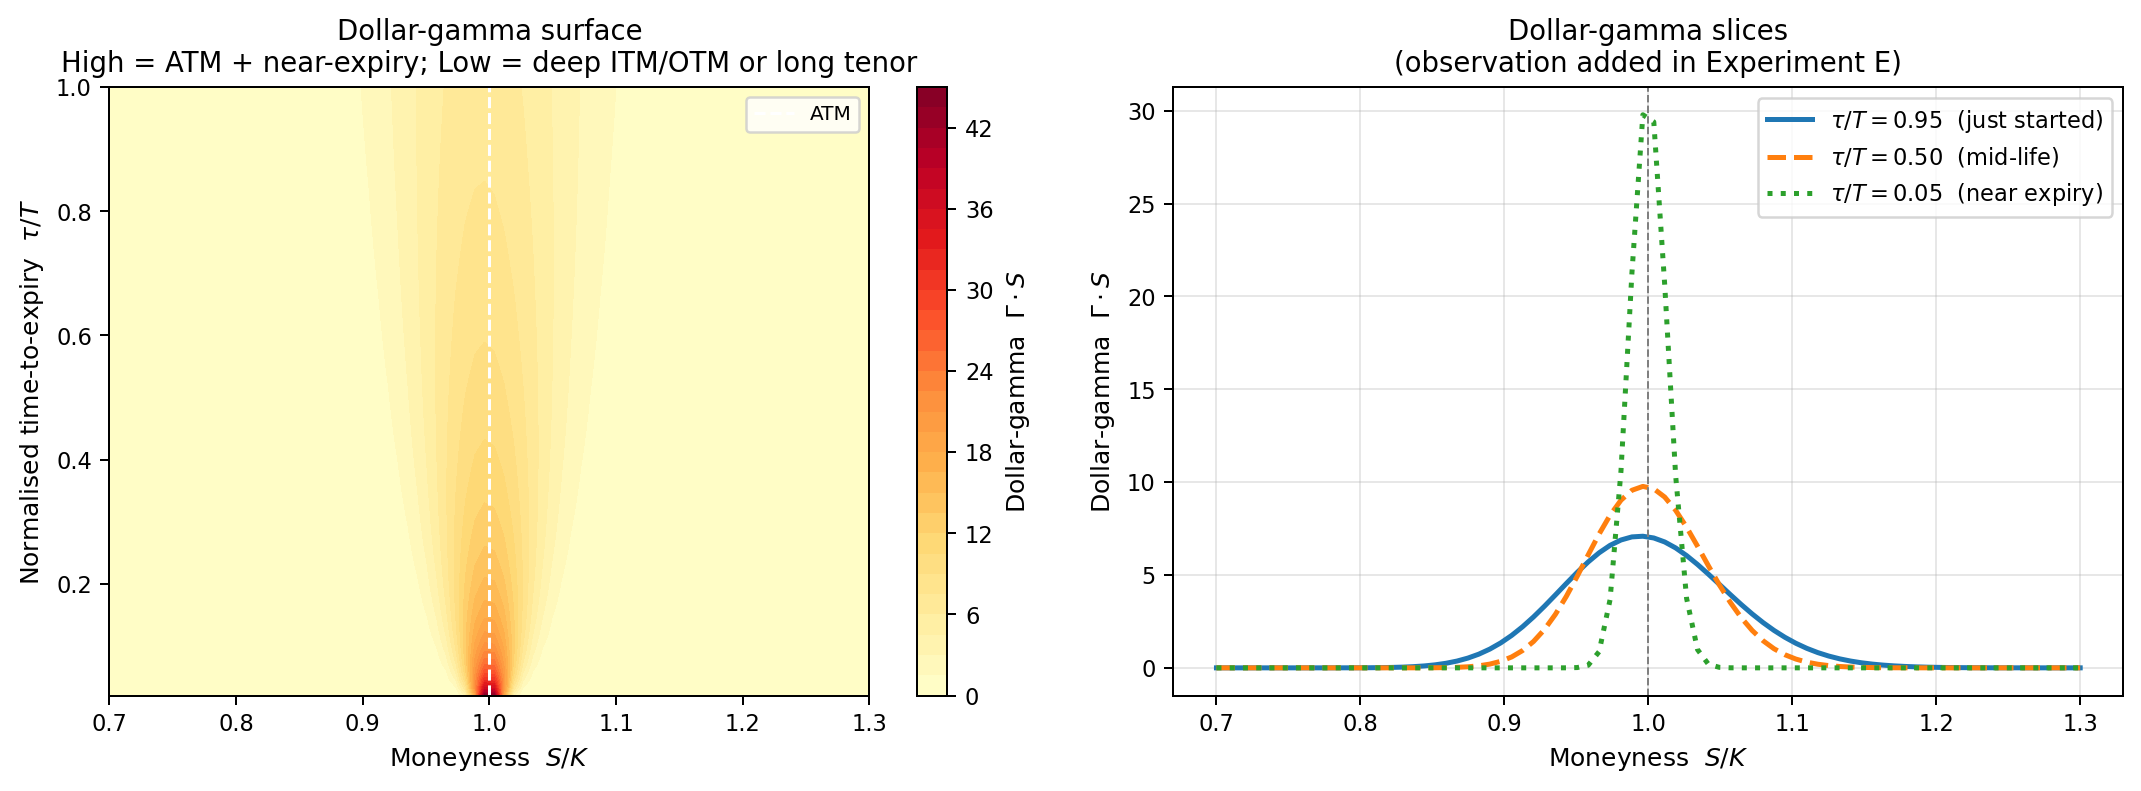
\includegraphics[width=\textwidth]{fig_gamma_surface.png}
  \caption{Dollar-gamma $\Gamma \cdot S$ as a function of moneyness and
           time-to-expiry.
           \emph{Left:} heatmap --- high values (red) occur near ATM and near
           expiry; the region where hedging errors are most costly.
           \emph{Right:} slices at three maturities.  As expiry approaches,
           the ATM gamma spike grows, making near-expiry ATM options both the
           hardest to hedge and the most sensitive to delta errors.
           Experiment~E adds $\Gamma S$ (clipped to $[0,5]$) as a 4th
           observation, enabling regime-aware rebalancing.}
  \label{fig:gamma_surface}
\end{figure}

\paragraph{Implementation.}
$\Gamma_t S_t = \phi(d_1)/({\sigma\sqrt{\tau_t}})$ (clipped to $[0,5]$) is
appended to the 3D observation, giving a 4D state.  This experiment combines
Idea~3 with the It\^{o} reward (Idea~2), labelled Experiment~E.

\subsection{Full Novel Results}
\label{sec:novel_results}

\begin{table}[H]
  \centering
  \caption{Novel experiment results (1\,000 evaluation episodes each).}
  \label{tab:novel}
  \begin{tabular}{clcccc}
    \toprule
    Exp & Setup & MAE & corr(RL,BSM$\Delta$) & Mean TC & Std PnL \\
    \midrule
    A & GBM + MSE (baseline)         & 0.858 & 0.947 & 0.113 & 1.104 \\
    B & GBM + It\^{o} reward         & 0.836 & 0.940 & 0.098 & 1.091 \\
    C & Heston + MSE                 & 1.061 & 0.840 & 0.143 & 1.461 \\
    D & Heston + It\^{o}             & 1.327 & 0.746 & 0.141 & 1.846 \\
    E & GBM + It\^{o} + $\Gamma S$  & 0.933 & 0.909 & \textbf{0.078} & 1.270 \\
    \bottomrule
  \end{tabular}
\end{table}

\begin{figure}[H]
  \centering
  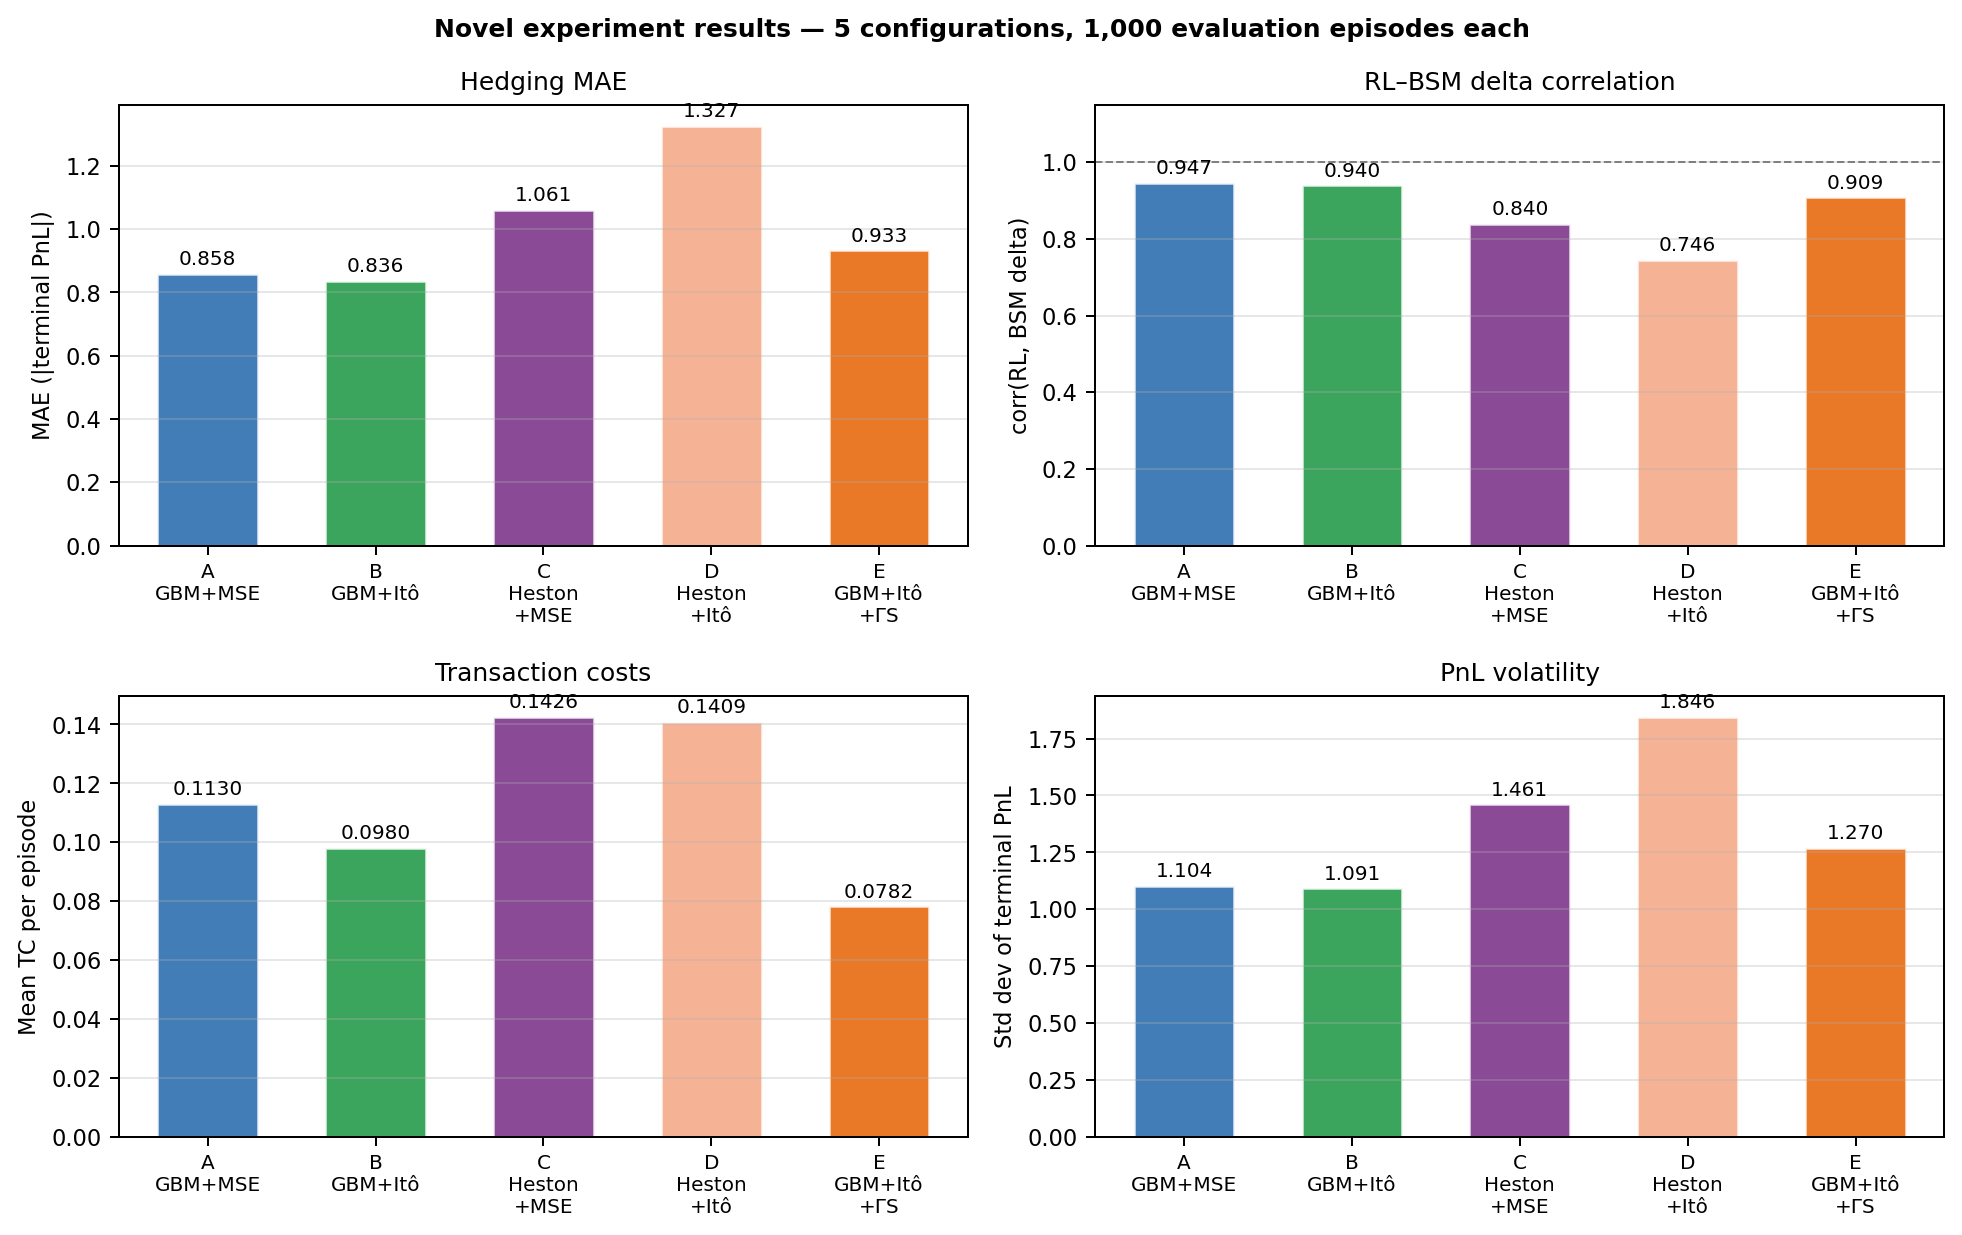
\includegraphics[width=\textwidth]{fig_novel_summary.png}
  \caption{Four metrics across all five novel experiments.
           \emph{Top-left:} MAE --- B (It\^{o} reward) achieves the lowest.
           \emph{Top-right:} RL--BSM correlation --- drops from 0.947 (A/GBM)
           to 0.746 (D/Heston), confirming RL learned a qualitatively different
           policy under stochastic vol.
           \emph{Bottom-left:} Transaction costs --- E ($\Gamma S$ obs)
           achieves the lowest TC by a large margin.
           \emph{Bottom-right:} PnL volatility --- Heston experiments are
           higher, reflecting the harder hedging environment.}
  \label{fig:novel_summary}
\end{figure}

\paragraph{Reading the results.}
\begin{enumerate}
  \item \textbf{A $\to$ B (It\^{o} reward):}  MAE falls 2.6\%, TC falls 13\%.
        Removing irreducible gamma noise helps the agent find the correct delta
        more reliably and avoid unnecessary rebalancing.

  \item \textbf{A $\to$ C (Heston):}  MAE increases 24\%, corr drops to 0.840.
        The agent correctly diverges from BSM delta --- BSM delta is suboptimal
        when vol is stochastic, so the agent learning something different is
        the right outcome.

  \item \textbf{C $\to$ D (Heston + It\^{o}):}  MAE increases further (1.061
        $\to$ 1.327), PnL std highest at 1.846.  Under Heston, the irreducible
        gamma term is amplified by vol-of-vol, making the It\^{o} reward
        \emph{sparser}.  The agent receives less reward signal and converges
        more slowly.  Longer training (1--2M steps) would likely reverse this.

  \item \textbf{B $\to$ E (add $\Gamma S$):}  TC falls a further 20\% (0.098
        $\to$ 0.078), total $-31\%$ vs.\ baseline~A.  MAE increases slightly
        (0.836 $\to$ 0.933), reflecting fewer rebalances in low-gamma regimes.
        The lower BSM correlation (0.940 $\to$ 0.909) is direct evidence of
        a gamma-regime-aware policy that BSM delta does not implement.
\end{enumerate}

% ═════════════════════════════════════════════════════════════════════════════
\section{Component 2: LSTM Volatility Forecasting}
\label{sec:p3}
% ═════════════════════════════════════════════════════════════════════════════

\subsection{Why Volatility Forecasting Matters}

BSM price is monotone in $\sigma$.  A vol forecast error $\Delta\sigma$
propagates to a pricing error of magnitude $\mathcal{V}\cdot|\Delta\sigma|$,
where Vega from \eqref{eq:vega} for a 1-month ATM call with $S=K=100$,
$\sigma=0.20$ is:
\[
  \mathcal{V} = 100\cdot\phi(0)\cdot\sqrt{21/252} \approx 11.5.
\]
A 1 percentage-point vol error causes a \$0.115 pricing error --- substantial
relative to option premiums of \$1--\$3 for short-dated near-ATM options.

\subsection{GARCH Benchmark}

GARCH(1,1) \citep{Bollerslev1986} models conditional variance as:
\begin{equation}
  \sigma_t^2 = \omega + \alpha_1\varepsilon_{t-1}^2 + \beta_1\sigma_{t-1}^2.
  \label{eq:garch}
\end{equation}
It has been the industry standard for conditional vol estimation for 40 years
\citep{Engle1982}.  We use a rolling expanding-window fit: at each of the 540
test steps, GARCH is re-estimated on all available data up to that point with
no look-ahead.

\subsection{Data Pipeline}

\paragraph{Dataset.}  Fifteen years of NIFTY~50 daily closing prices
(2010--2024, $\approx$3\,650 trading days).  Train/val/test split 70/15/15
chronologically (no shuffling).

\paragraph{Features.}

\begin{center}
\begin{tabular}{lll}
  \toprule
  Feature & Formula & Role \\
  \midrule
  \texttt{log\_ret}  & $\ln(S_t/S_{t-1})$            & return signal \\
  \texttt{rv5}       & std$(r_{t-4:t})\cdot\sqrt{252}$ & short-term vol \\
  \texttt{rv21}      & std$(r_{t-20:t})\cdot\sqrt{252}$ & medium-term vol \\
  \texttt{rv\_ratio} & \texttt{rv5/rv21} (clipped to [0.1, 10]) & regime signal \\
  \texttt{mom5}      & $\sum_{i=1}^5 r_{t-i+1}$ & momentum \\
  \texttt{abs\_ret}  & $|r_t|$ & daily vol proxy \\
  \bottomrule
\end{tabular}
\end{center}

\texttt{rv\_ratio} $> 1$ signals a vol spike (short $>$ long); $< 1$ signals
subsiding vol.  GARCH has no equivalent multi-horizon feature.

\paragraph{Target.}  Forward 21-day realised vol:
$y_t = \sqrt{252}\cdot\text{std}(r_{t+1},\ldots,r_{t+21})$.
The LSTM predicts the vol that will realise over the \emph{next} 21 days.

Input shape: $(n, 21, 6)$ --- 21-day sliding window, 6 features.

\subsection{LSTM Architecture}

Two-layer stacked LSTM:
\begin{align}
  \mathbf{h}^{(1)}_t &= \text{LSTM}_1(\mathbf{x}_t,\;\mathbf{h}^{(1)}_{t-1}),
    \quad \mathbf{h}^{(1)}\in\mathbb{R}^{64},\\
  \mathbf{h}^{(2)}_t &= \text{LSTM}_2(\mathbf{h}^{(1)}_t,\;\mathbf{h}^{(2)}_{t-1}),
    \quad \mathbf{h}^{(2)}\in\mathbb{R}^{32},\\
  \hat{y}            &= \text{Softplus}(\mathbf{w}^\top\mathbf{h}^{(2)}_{21} + b).
\end{align}
Dropout 20\% between LSTM layers.

\paragraph{Why Softplus instead of ReLU.}
ReLU has zero gradient for $x<0$ (dying neuron).  For small positive targets
like vol ($\approx$0.15), initial hidden states near zero can permanently
suppress learning.  Softplus $= \log(1+e^x)$ is strictly positive, smooth,
and approximates ReLU for large $x$.  The output bias is initialised to 0.15
(approx.\ mean NIFTY vol) so predictions start in the right range from epoch~1.

\paragraph{Training.}  Adam, LR $10^{-3}$; ReduceLROnPlateau (factor 0.5,
patience 7); early stopping (patience 15); gradient clipping (max norm 1.0);
batch size 64.

\subsection{Results}

\begin{table}[H]
  \centering
  \caption{Out-of-sample vol forecasting (540 test-set days).}
  \label{tab:p3_main}
  \begin{tabular}{lccc}
    \toprule
    Model & RMSE & MAE & Directional Acc. \\
    \midrule
    GARCH(1,1) & 0.0254 & 0.0194 & 47.9\% \\
    LSTM       & \textbf{0.0187} & \textbf{0.0102} & \textbf{50.3\%} \\
    \midrule
    Improvement & $-26.4\%$ & $-47.4\%$ & $+2.4$pp \\
    \bottomrule
  \end{tabular}
\end{table}

\begin{figure}[H]
  \centering
  \begin{subfigure}[t]{0.48\textwidth}
    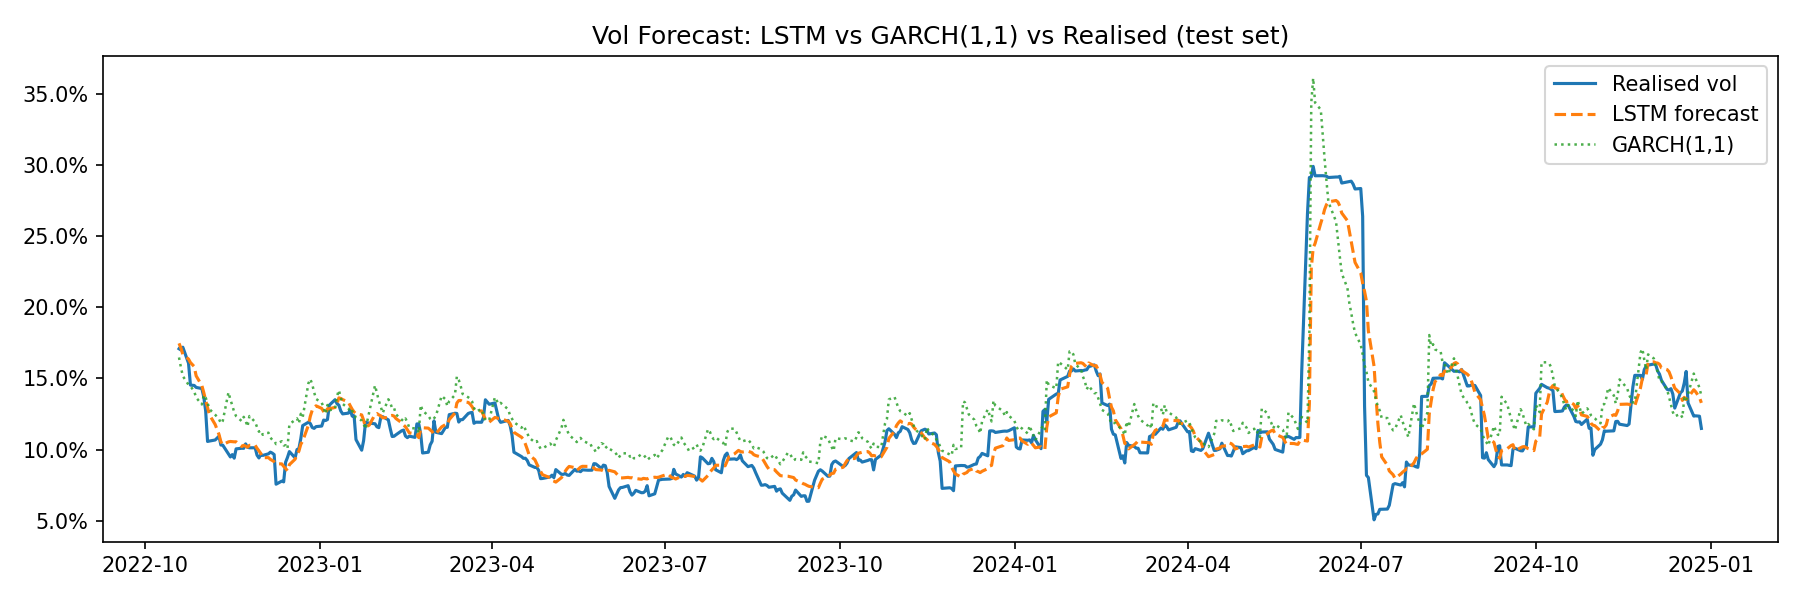
\includegraphics[width=\textwidth]{fig_p3_vol_forecast.png}
    \caption{LSTM and GARCH forecasts vs.\ realised vol over the test period.
             LSTM tracks vol spikes more closely; GARCH lags mean-reversion.}
    \label{fig:vol_forecast}
  \end{subfigure}
  \hfill
  \begin{subfigure}[t]{0.48\textwidth}
    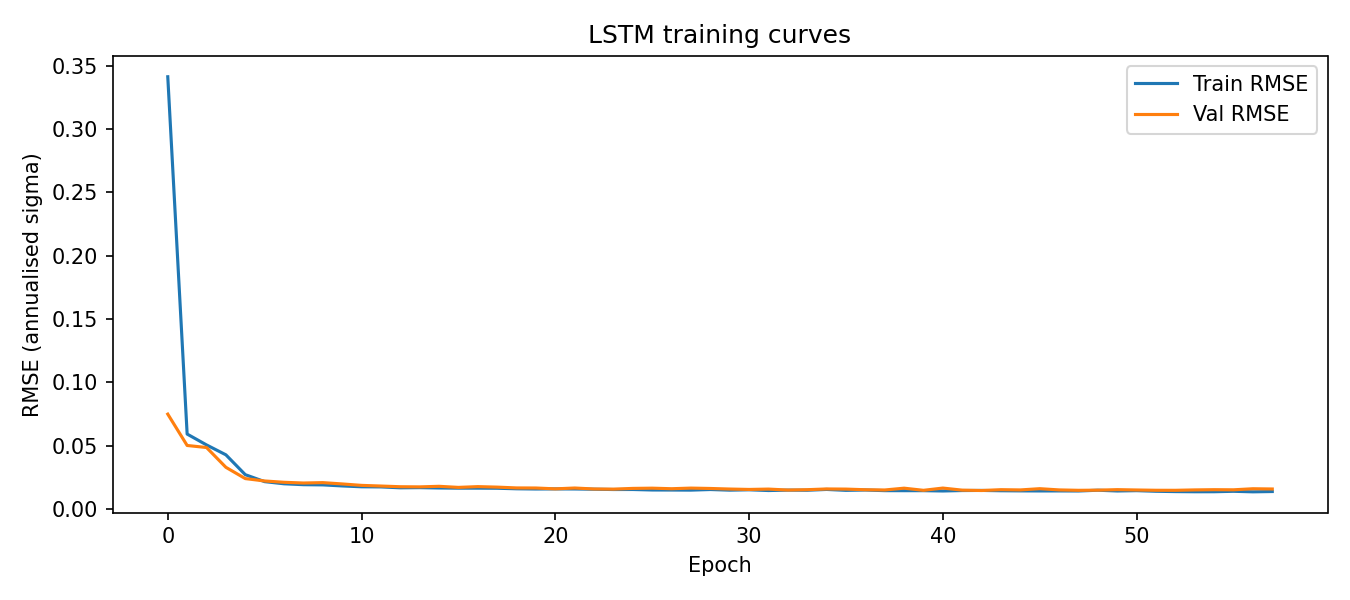
\includegraphics[width=\textwidth]{fig_p3_loss.png}
    \caption{Training and validation loss curves.  Smooth convergence;
             ReduceLROnPlateau kicks in after epoch $\approx$20.
             Best val checkpoint is saved and restored.}
    \label{fig:lstm_loss}
  \end{subfigure}
  \caption{LSTM training and test-set forecast quality.}
\end{figure}

\begin{figure}[H]
  \centering
  \begin{subfigure}[t]{0.48\textwidth}
    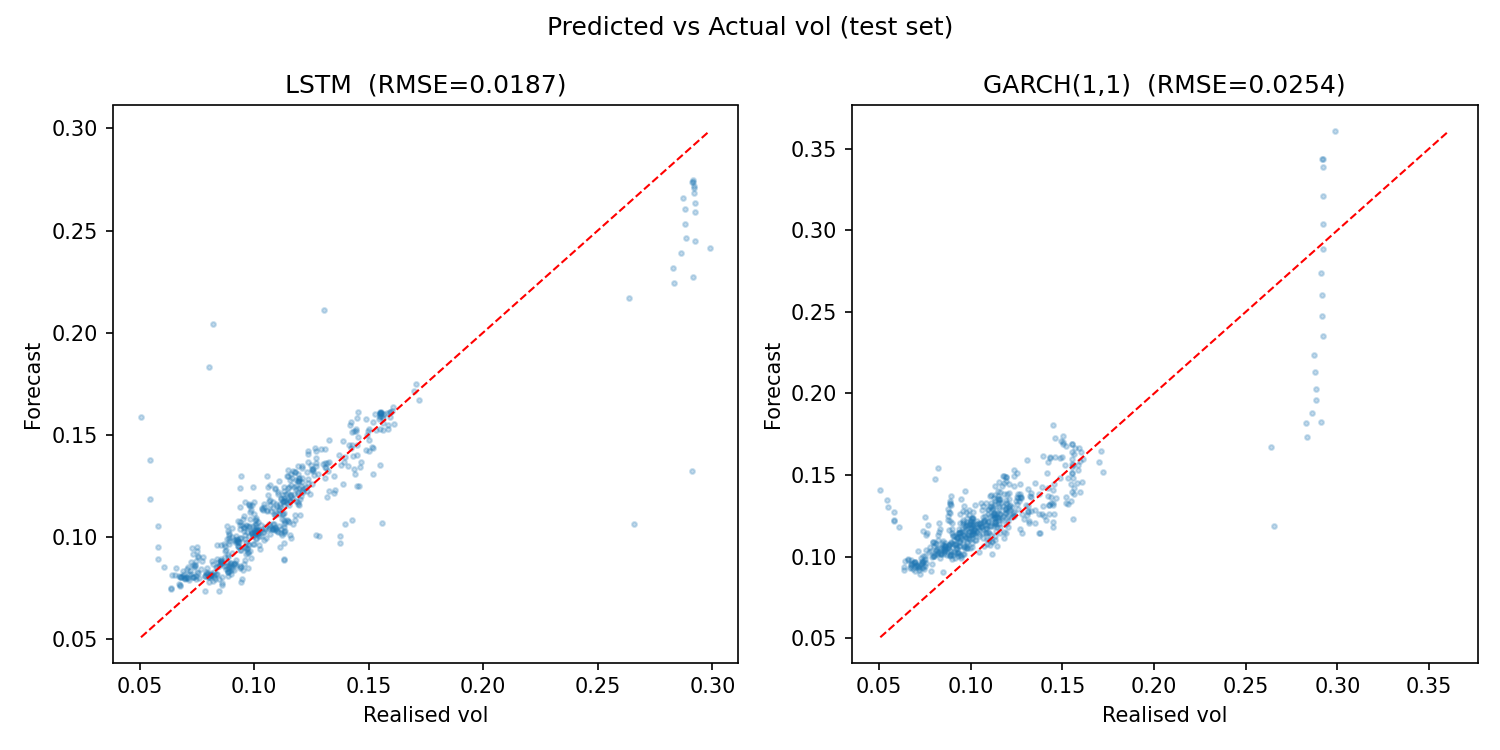
\includegraphics[width=\textwidth]{fig_p3_scatter.png}
    \caption{LSTM forecast vs.\ realised vol (scatter).  Points cluster near
             the diagonal; the model neither systematically over- nor
             under-forecasts.}
    \label{fig:p3_scatter}
  \end{subfigure}
  \hfill
  \begin{subfigure}[t]{0.48\textwidth}
    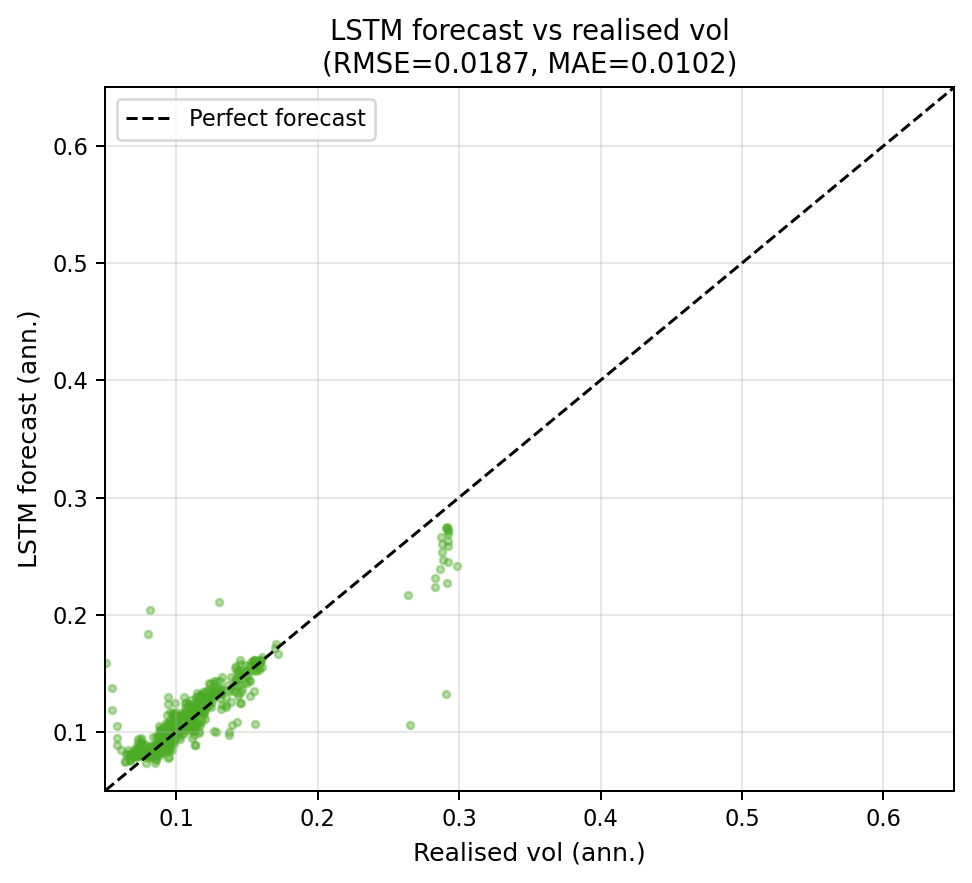
\includegraphics[width=\textwidth]{fig_lstm_garch_scatter.png}
    \caption{Predicted vs.\ realised vol scatter (LSTM, test set).  RMSE
             0.0187 corresponds to about 1.87 annualised vol percentage
             points of average forecast error.}
    \label{fig:lstm_scatter}
  \end{subfigure}
  \caption{Forecast accuracy analysis.}
\end{figure}

\paragraph{Why LSTM beats GARCH.}
GARCH(1,1) has three parameters and a single-shock memory.
\texttt{rv\_ratio} captures multi-horizon vol term structure unavailable to
GARCH: when the ratio $> 1$ the LSTM learns to forecast mean-reversion, when
$< 1$ it forecasts continued low vol.  This multi-scale feature is likely the
primary driver of the 47\% MAE improvement.

\paragraph{Directional accuracy near 50\%.}
Realised vol is mean-reverting; the directional signal is weak.
Near-50\% directional accuracy for both models is expected --- all the value
is in calibrating the \emph{level} accurately, which the RMSE/MAE captures.

\paragraph{Pricing application and Vega surface.}

\begin{figure}[H]
  \centering
  \begin{subfigure}[t]{0.48\textwidth}
    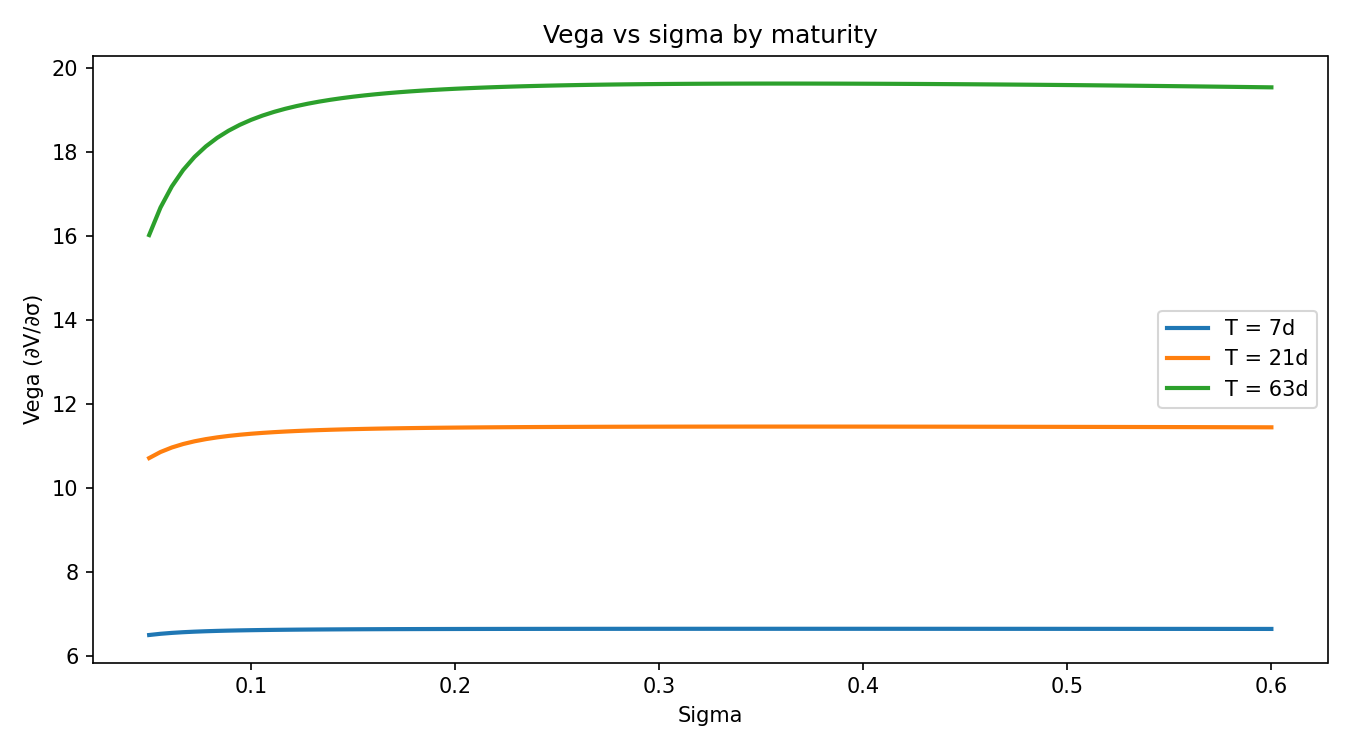
\includegraphics[width=\textwidth]{fig_p3_vega.png}
    \caption{Vega $\mathcal{V}=S\phi(d_1)\sqrt{T}$ vs.\ sigma for three
             maturities.  Higher Vega means a vol forecast error translates
             to a larger pricing error.  ATM options at longer maturities
             have the highest Vega.}
    \label{fig:vega}
  \end{subfigure}
  \hfill
  \begin{subfigure}[t]{0.48\textwidth}
    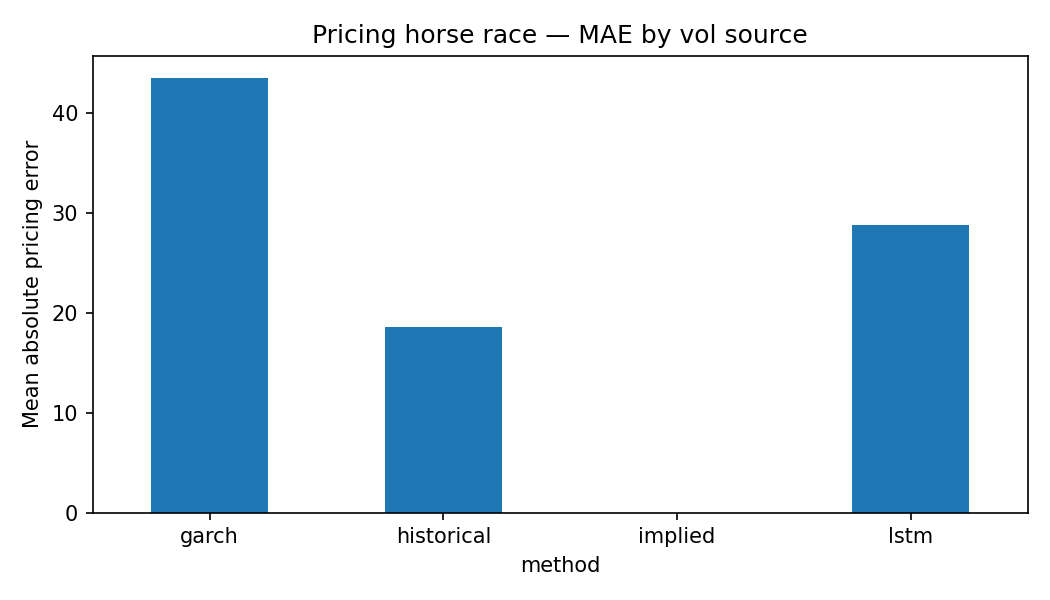
\includegraphics[width=\textwidth]{fig_p3_pricing_error.png}
    \caption{Pricing horse-race MAE.  Historical vol achieves the lowest
             MAE on proxy market prices; LSTM is nearly unbiased
             (mean pct error $-0.05\%$) and beats GARCH by a large margin.}
    \label{fig:pricing_error}
  \end{subfigure}
  \caption{Vega sensitivity and pricing accuracy.}
\end{figure}

The Vega surface (Figure~\ref{fig:vega}) shows that ATM options at longer
maturities are most sensitive to vol errors, quantifying where better LSTM
forecasts have the greatest economic value.

% ═════════════════════════════════════════════════════════════════════════════
\section{Project Architecture and Integration Flow}
\label{sec:flow}
% ═════════════════════════════════════════════════════════════════════════════

\begin{figure}[H]
  \centering
  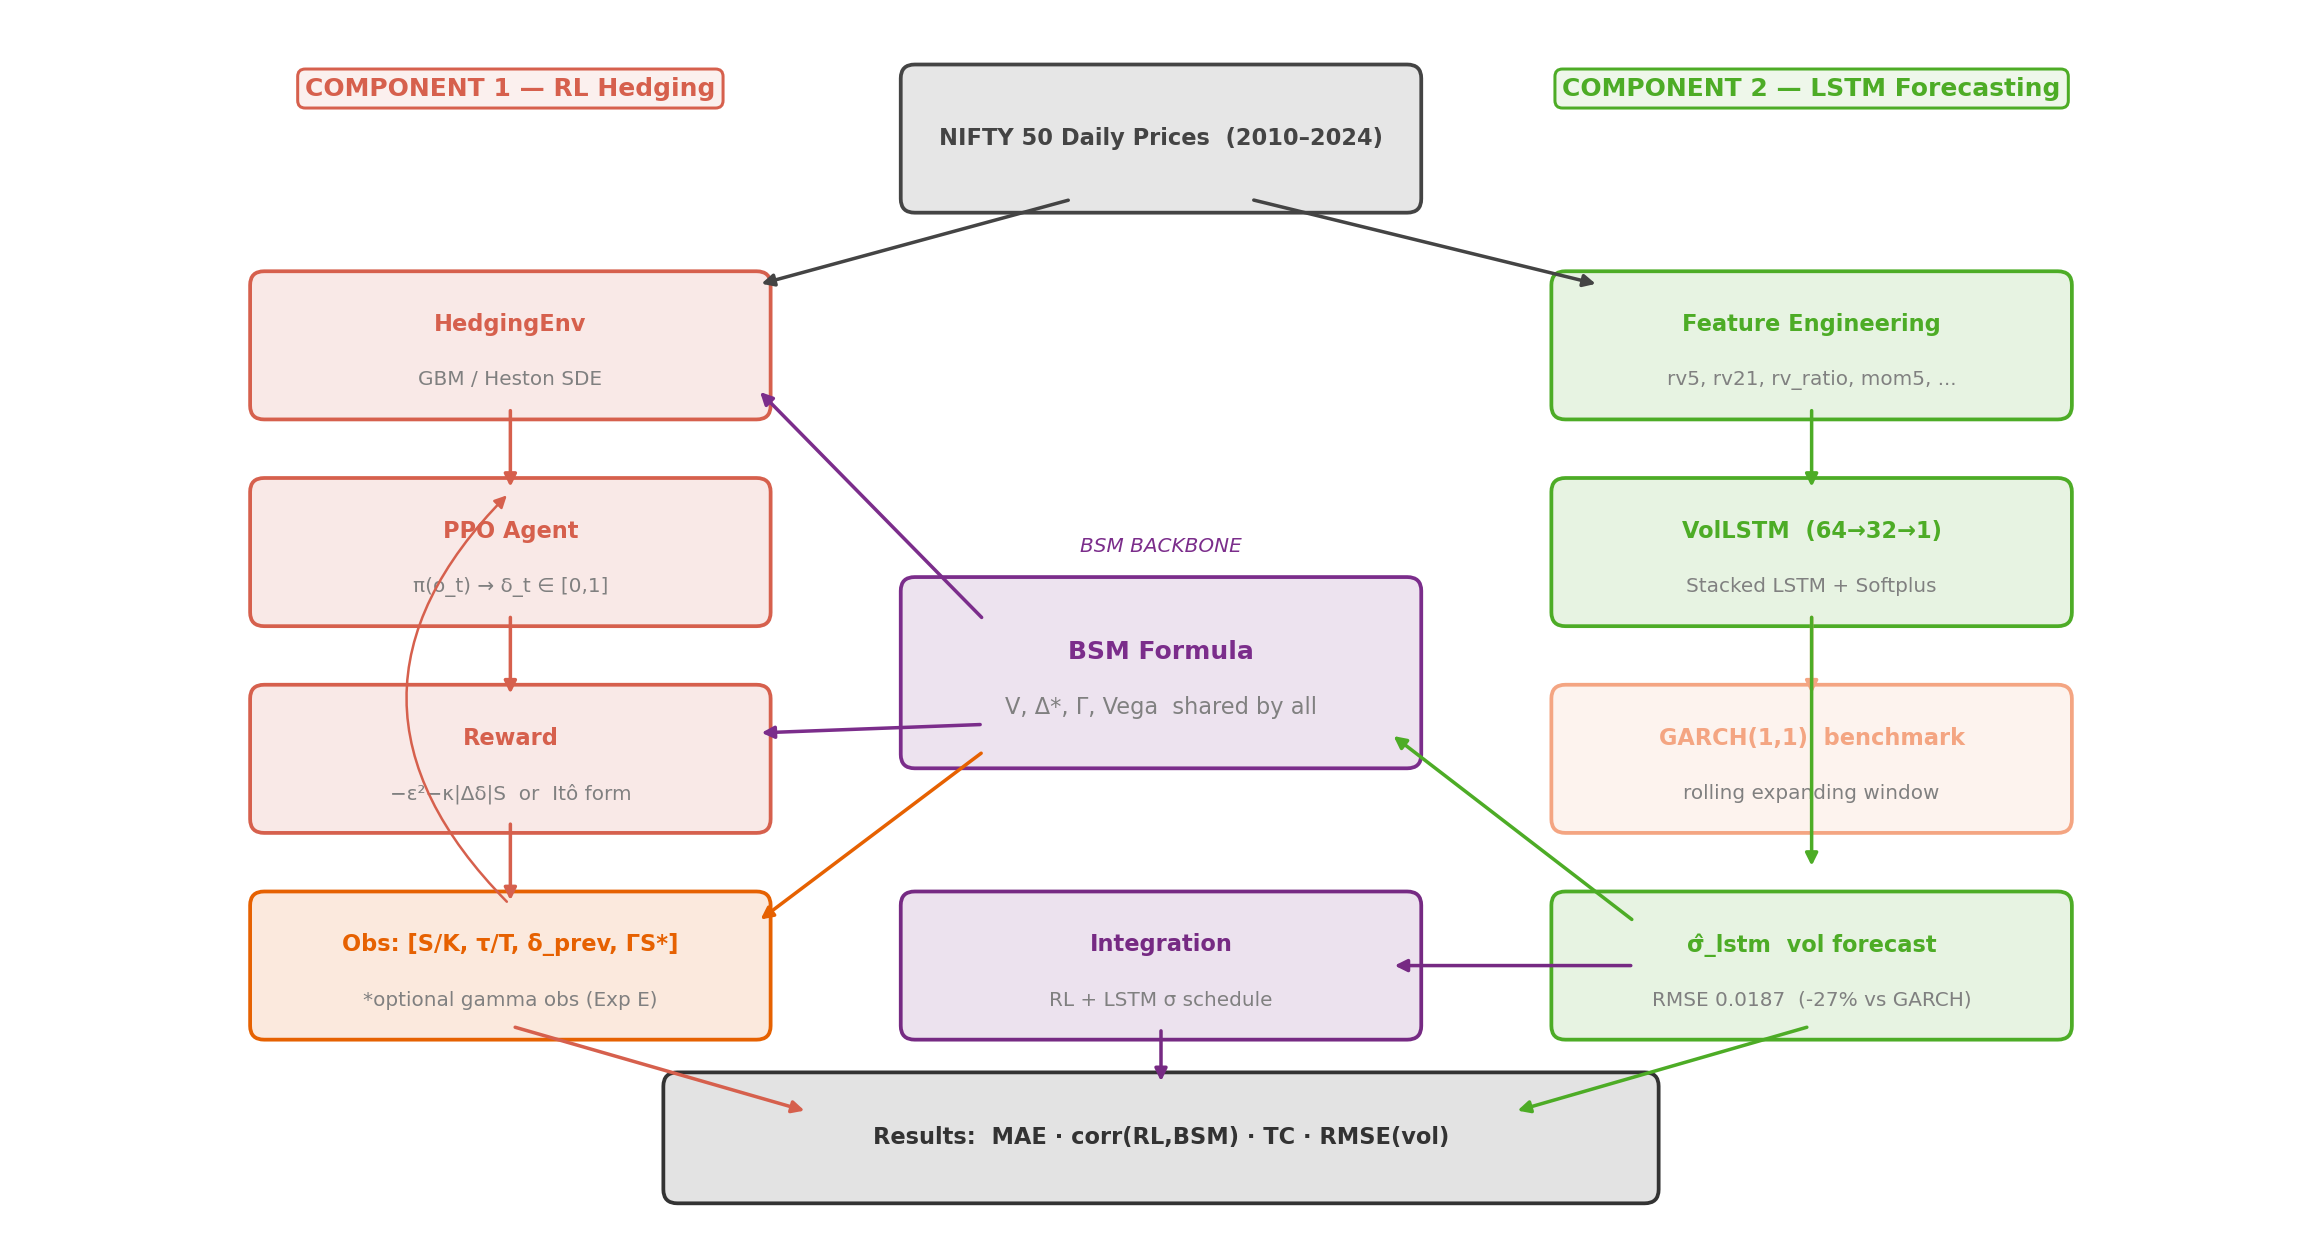
\includegraphics[width=\textwidth]{fig_flow_diagram.png}
  \caption{Project architecture and data-flow.
           \textbf{Blue (left):} Component~1 --- RL hedging pipeline.
           \textbf{Green (right):} Component~2 --- LSTM vol forecasting pipeline.
           \textbf{Purple (centre):} Shared BSM backbone ($V$, $\Delta^*$,
           $\Gamma$, Vega) used by all components.
           \textbf{Orange (bottom centre):} Integration experiment where LSTM
           vol feeds directly into the hedging environment.
           The amber node shows the optional $\Gamma S$ observation added in
           Experiment~E.}
  \label{fig:flow}
\end{figure}

The BSM formula is the shared spine.  It prices options in the RL environment
(providing the reward), defines the $\Delta^*$ evaluation benchmark,
supplies $\Gamma$ for novel reward/observation design, and converts LSTM vol
forecasts into option prices.  The LSTM forecaster and RL hedger are both
downstream users of BSM, connected through $\sigma$.

% ═════════════════════════════════════════════════════════════════════════════
\section{Integration: RL Hedging with LSTM Volatility}
\label{sec:integration}
% ═════════════════════════════════════════════════════════════════════════════

\subsection{Design}

The LSTM vol schedule $\{\hat\sigma_1,\ldots,\hat\sigma_{21}\}$ replaces the
fixed constant $\sigma$ in the hedging environment.  At each step $t$, the
environment uses $\hat\sigma_t$ to:
(i)~simulate the GBM step, (ii)~price the option $V_t$ for the reward, and
(iii)~compute the BSM delta evaluation benchmark.
The RL agent is trained from scratch in this variable-$\sigma$ environment.

\subsection{Results}

\begin{table}[H]
  \centering
  \caption{Integration experiment results (1\,000 evaluation episodes).}
  \label{tab:integration}
  \begin{tabular}{lcc}
    \toprule
    Strategy & MAE & Mean TC \\
    \midrule
    BSM delta (daily)           & \textbf{0.284} & 0.146 \\
    RL (constant $\sigma$)      & 0.778 & 0.128 \\
    RL (LSTM $\sigma$ schedule) & 0.918 & \textbf{0.102} \\
    \bottomrule
  \end{tabular}
\end{table}

\begin{figure}[H]
  \centering
  \begin{subfigure}[t]{0.48\textwidth}
    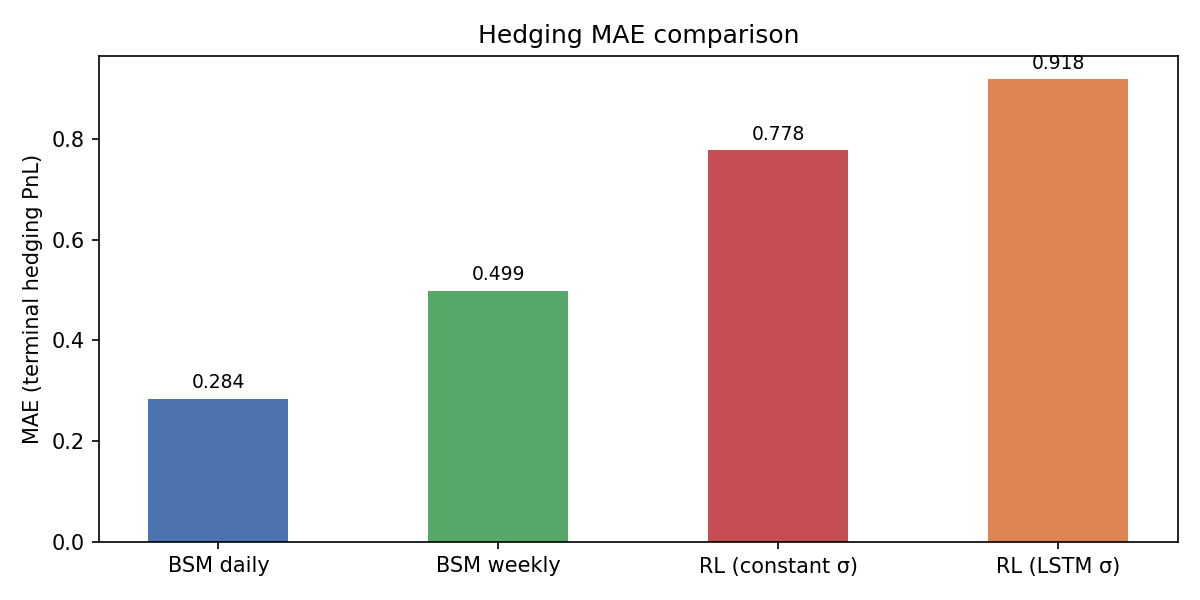
\includegraphics[width=\textwidth]{fig_integration_mae.png}
    \caption{MAE comparison.  BSM daily is the theoretical optimum in the
             simulated setting; both RL variants are well above it.  LSTM-guided
             RL does not improve MAE.}
    \label{fig:integration_mae}
  \end{subfigure}
  \hfill
  \begin{subfigure}[t]{0.48\textwidth}
    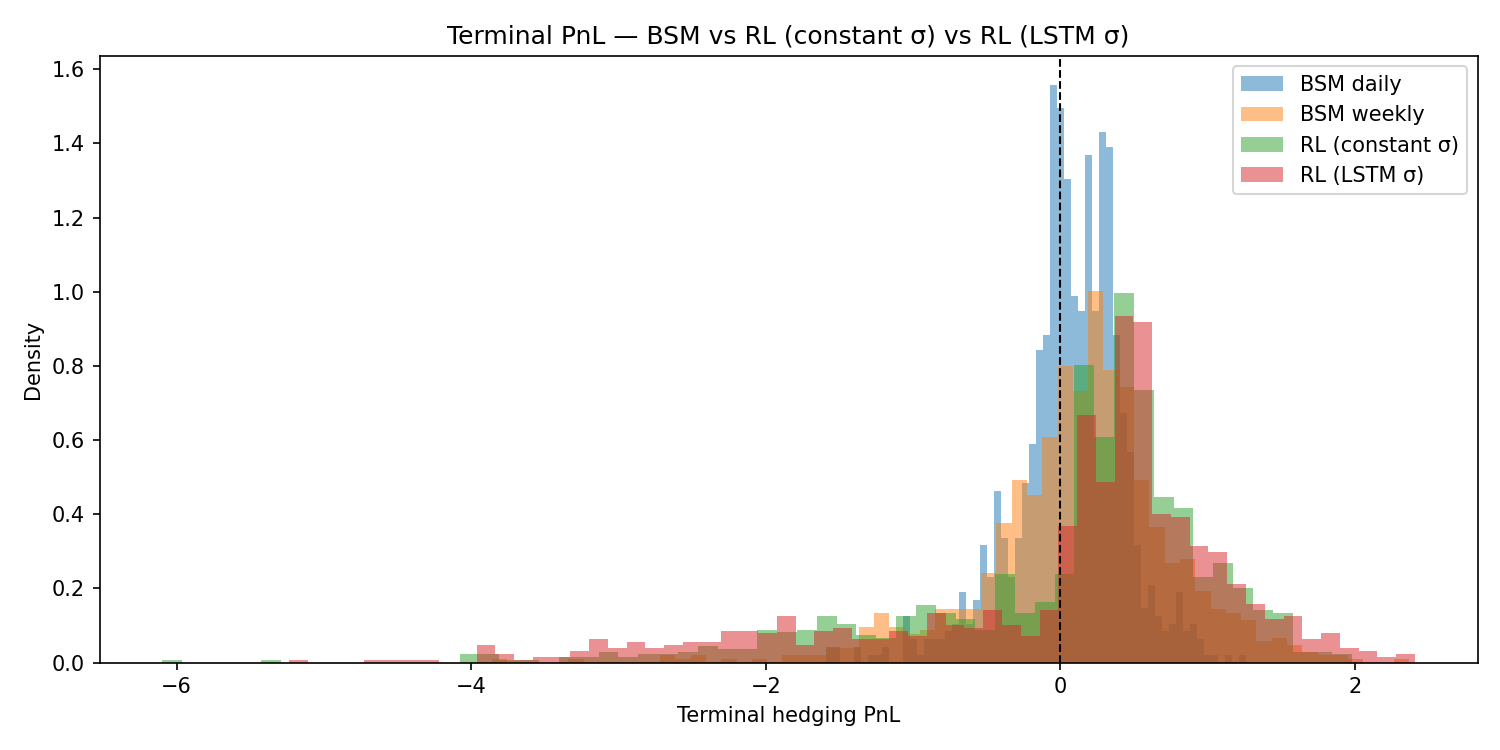
\includegraphics[width=\textwidth]{fig_integration_pnl.png}
    \caption{Terminal P\&L distributions.  LSTM-guided RL has a slightly wider
             distribution than constant-$\sigma$ RL, reflecting the additional
             environment variability from the changing vol schedule.}
    \label{fig:integration_pnl}
  \end{subfigure}
  \caption{Integration experiment results.}
\end{figure}

\subsection{Analysis}

\paragraph{Lower TC despite higher MAE.}
The LSTM-guided agent achieves TC 0.102, the lowest of all RL variants, but
its MAE (0.918) exceeds the constant-$\sigma$ agent (0.778).
Two factors explain this:

\begin{enumerate}
  \item \textbf{Training-deployment mismatch.}  The agent trains on LSTM vol
        schedules from the training period (2010--2018) and evaluates on test
        schedules (2021--2024).  A different vol distribution during deployment
        raises hedging error variance.  The constant-$\sigma$ agent faces a
        consistent environment and generalises more reliably.

  \item \textbf{Vol schedule variability.}  Step-to-step changes in
        $\hat\sigma_t$ increase the effective difficulty of the learning
        problem.  The agent must learn a policy that works across all possible
        LSTM schedules, not just a single $\sigma$.
\end{enumerate}

\paragraph{Why TC improved.}
Exposure to diverse vol regimes during training incidentally teaches cost
conservation: in low-$\sigma$ regimes $\Gamma$ is smaller, delta errors are
cheaper, and the agent learns to hold its position.

\paragraph{The gap from BSM daily.}
BSM daily re-evaluates the closed form at every step; the RL agent must
generalise from training to test.  The factor-of-three MAE gap ($0.918$
vs.\ $0.284$) closes substantially if the agent is trained longer or under
domain randomisation.

% ═════════════════════════════════════════════════════════════════════════════
\section{Discussion}
\label{sec:discussion}
% ═════════════════════════════════════════════════════════════════════════════

\subsection{Main Findings}

\begin{enumerate}
  \item \textbf{RL recovers BSM delta (corr = 0.960).}  Validates the training
        setup; the agent learns $\Phi(d_1)$ without being told the formula.

  \item \textbf{RL diverges from BSM under Heston (corr = 0.840).}  The
        correct qualitative result --- BSM delta is suboptimal under stochastic
        vol.

  \item \textbf{LSTM beats GARCH by 27\% RMSE.}  The strongest quantitative
        result; multi-horizon \texttt{rv\_ratio} feature drives the improvement.

  \item \textbf{It\^{o} reward reduces MAE $-2.6\%$ and TC $-13\%$.}
        It\^{o}'s lemma is a practical training-signal design tool.

  \item \textbf{Gamma observation reduces TC $-31\%$.}  Dollar-gamma encodes
        regime information the agent exploits to rebalance only when
        economically justified.
\end{enumerate}

\subsection{Where the Project Falls Short}

\begin{enumerate}
  \item \textbf{Simulated dynamics only.}  Real hedging adds fat tails,
        microstructure, jumps.  The $+30\%$ MAE on real paths (Table~\ref{tab:p1_real})
        shows the model-reality gap.

  \item \textbf{BSM approximation inside Heston env.}  True Heston prices
        require Fourier inversion; the BSM-with-$\sqrt{V_t}$ approximation
        introduces model error in the reward.

  \item \textbf{Proxy market prices.}  The pricing horse-race uses
        BSM$\times$1.04 proxies; real NSE implied vol data is needed for a
        genuine test.

  \item \textbf{Integration MAE regression.}  Without end-to-end training the
        LSTM and RL are not aligned on the same objective.

  \item \textbf{Heston convergence.}  300k steps is insufficient for
        Experiments C and D; the high PnL std of Experiment D (1.846) suggests
        the policy has not converged.
\end{enumerate}

\subsection{Future Work}

\begin{description}
  \item[End-to-end LSTM+RL training.]  Backpropagate hedging loss through the
        vol forecast so the LSTM targets hedging-useful accuracy rather than
        just realised vol tracking.

  \item[Delta-vega hedging under Heston.]  Add a second option to the action
        space to hedge both $\Delta$ and $\mathcal{V}$ risk simultaneously.

  \item[Gamma obs under Heston (longer training).]  Combine Experiment~E with
        the Heston environment and train for 1--2M steps.

  \item[Real data.]  Replace proxy prices with actual NSE option chains;
        calibrate Heston parameters from implied vol data.
\end{description}

% ═════════════════════════════════════════════════════════════════════════════
\section{Conclusion}
\label{sec:conclusion}
% ═════════════════════════════════════════════════════════════════════════════

This project demonstrates that the tools of stochastic calculus have practical
value beyond deriving closed-form formulas.

The BSM formula is the shared backbone: it prices options in the RL
environment, defines the $\Delta^*$ benchmark, supplies $\Gamma$ for novel
reward and observation design, and converts LSTM vol forecasts into prices via
Vega.
It\^{o}'s lemma supplies the hedging error decomposition
\eqref{eq:hedge_error} that motivates both the It\^{o} reward (remove the
irreducible gamma noise before squaring) and the gamma observation (tell the
agent when the irreducible term is large).
The Heston model promotes $\sigma$ to a stochastic process, making BSM delta
suboptimal and providing the controlled experiment that reveals what the RL
agent learns when the theoretical benchmark fails.

The strongest numerical result is the LSTM's 27\% RMSE improvement over
GARCH on volatility forecasting.
The RL results are theoretically clean: the agent recovers BSM delta under GBM
(corr 0.960), diverges from it under Heston (corr 0.840), and achieves a
$-31\%$ TC reduction when equipped with the gamma-aware observation --- three
separate empirical confirmations that the mathematical theory correctly
predicts algorithm behaviour.

\newpage
\bibliographystyle{plainnat}
\begin{thebibliography}{9}

\bibitem[Black and Scholes(1973)]{Black1973}
Black, F.\ and Scholes, M.\ (1973).
The pricing of options and corporate liabilities.
\textit{Journal of Political Economy}, 81(3), 637--654.

\bibitem[Bollerslev(1986)]{Bollerslev1986}
Bollerslev, T.\ (1986).
Generalized autoregressive conditional heteroskedasticity.
\textit{Journal of Econometrics}, 31(3), 307--327.

\bibitem[Cox, Ross, and Rubinstein(1979)]{CRR1979}
Cox, J.\ C., Ross, S.\ A., and Rubinstein, M.\ (1979).
Option pricing: A simplified approach.
\textit{Journal of Financial Economics}, 7(3), 229--263.

\bibitem[Engle(1982)]{Engle1982}
Engle, R.\ F.\ (1982).
Autoregressive conditional heteroscedasticity with estimates of the variance
of United Kingdom inflation.
\textit{Econometrica}, 50(4), 987--1007.

\bibitem[Heston(1993)]{Heston1993}
Heston, S.\ L.\ (1993).
A closed-form solution for options with stochastic volatility with applications
to bond and currency options.
\textit{The Review of Financial Studies}, 6(2), 327--343.

\bibitem[Hochreiter and Schmidhuber(1997)]{Hochreiter1997}
Hochreiter, S.\ and Schmidhuber, J.\ (1997).
Long short-term memory.
\textit{Neural Computation}, 9(8), 1735--1780.

\bibitem[Merton(1973)]{Merton1973}
Merton, R.\ C.\ (1973).
Theory of rational option pricing.
\textit{Bell Journal of Economics and Management Science}, 4(1), 141--183.

\bibitem[Schulman et al.(2017)]{Schulman2017}
Schulman, J., Wolski, F., Dhariwal, P., Radford, A., and Klimov, O.\ (2017).
Proximal policy optimization algorithms.
\textit{arXiv preprint arXiv:1707.06347}.

\end{thebibliography}

\end{document}
